
\chapter{Finite Element Methods for the shallow water equations}
\label{eulerian_sw}


Due to the complexity of the geometry and the source terms is not possible to find an analytical solution for the SW equations, this explains the need to design strategies to find numerical solutions. In this chapter some numerical strategies with the FEM in an eulerian framework are explored.
The Eulerian frameworks are robust and very efficient for continuous problems. However, discontinuities and front tracking may require especial attention. Since in those physical phenomena flooding or moving shoreline may occur, the identification of the dry domain is a challenging problem for the Eulerian FEM.
Moreover, monotonic properties are especially interesting when partially wet domains are considered, since the water depth is a positive magnitude but, in general, numerical methods does not verify this property.

The SW equations have traditionally been modelled using finite volumes (FV) because of its advantages of stability and monotonicity. Given its geometric flexibility and its natural way to introduce high order schemes, the FEM has been applied too \cite{zien3,navon1979,navon1988}.
Halfway between FV and FEM, there is the discontinuous Galerkin (DG) technique \cite{ambati2007,khan2014,lee2019}. DG method has the advantages of the geometrical flexibility of the FEM and the stability of FV, but the introduction of high order DG schemes is not straightforward.
Since the FEM can exhibit spurious oscillations, different strategies such as stabilization, monotonic schemes or different order of polynomial interpolation can be explored \cite{hood1974,zien3,ortiz2012}.




%This research is focused in classical stabilized finite elements with an equal order interpolation for all the variables. We will explore the capabilities of the finite increment calculus (FIC) technique to develop stable formulations for the SW equations.

In this chapter, the general procedure for FEM is presented. Then, some stabilization techniques are explored: the FIC-based stabilization, the flux corrected technique and the gradient jump viscosity method. Finally, the stabilized formulation is applied to the Boussinesq modified equations. Several examples are provided to show the capabilities and limitations of each method.




\section{Galerkin weak formulation}



We consider a balance equation in the space domain $\Omega$ and the time interval $[0,T]$. Let $\bm{\phi}$ and $\bm{\psi}$ be vector functions of the domain $\Omega \times [0,T]$ and $\mathbf{r}$ the residual of the balance equations expressed in terms of the unknown $\bm{\phi}$.
The space of functions that are square-integrable in $\Omega$ is denoted as $L^2(\Omega)$. And the space of functions whose derivatives up to order $m\geq0$ belong to $L^2(\Omega)$ is denoted by $H^m(\omega)$. The space $H_0^1(\Omega)$ consists on a subspace of $H^1(\Omega)$ vanishing on $\partial \Omega$.

Using this notation, the space of functions for the continuous problem are $V \defeq H^1(\Omega)$ and for the test functions $V_0 \defeq H_0^1(\Omega)$.
The variational form of the balance equations can be expressed as find $\bm{\phi} \in V$ such that $\forall \bm{\psi} \in V_0$
\begin{equation} \label{variational_form}
    \int_\Omega \bm{\psi} \cdot \mathbf{r}(\bm{\phi}) \ d\Omega = 0
\end{equation}



The standard Galerkin approximation \ref{variational_form} is straightforward. Let $\mathcal{P}_h$ be a partition of the domain $\Omega$. The diameter of an element domain $e\in\mathcal{P}_h$ is denoted by $l_e$. From the polynomial spaces defined by the finite elements, we can construct the subspaces $V_h\in V$ and $V_{h,0}\in V_0$. The Galerkin approximation of the balance equations can be expressed as find $\bm{\phi}_h \in V_h$ such that $\forall \bm{\psi} \in V_{h,0}$
\begin{equation} \label{discrete_variational}
    \int_\Omega \bm{\psi} \cdot \mathbf{r}(\bm{\phi}) \ d\Omega = 0
\end{equation}

Unfortunately, this problem is not straightforward to solve using finite elements, as its discrete version is not numerically stable. In fact, to ensure that the problem of finding $\bm{\phi}$ has a stable solution, the space must verify the inf-sub condition \cite{codina2011}.



\section{Stabilized formulations for the shallow water equations}
\label{sec:fic_fem_stabilization}


Several families of stabilization methods can be found in the literature, usually applied to the convection-diffusion equations and the Navier-Stokes equations. The most relevant are SUPG \cite{brooks1982},
ASGS\cite{codina1998}, GLS \cite{hughes1989} and FIC\cite{onate1996,onate1998}.
Due to the hyperbolic character of the SW equations, a particular stabilization method for compressible flow or the Euler equations need to be developed.
The FIC approach is based on the incremental solution of a modified system of non-local governing equations accounting for higher order terms obtained by applying the balance laws in domains of finite size.
The FIC-based stabilization has been applied in conjunction with the FEM to convection-diffusion, incompressible flows, among other applications \cite{onate1998,onate2001}.
In those cases, where the convective term has an important role, a first order FIC term is enough to provide stability to the system.
However, the SW equations are governed by the convective term and the wave equation in a mixed formulation \cite{codina2008}. In consequence, the common derivation of the FIC-based stabilization is not enough to provide stability in all the range of applicability of the SW equations. 
A generalization of this method is proposed in order to provide a global stability for the SW equations.

Once global stability is achieved, local instabilities may appear near discontinuities, which are inherent to the supercritical flows.
A local shock capturing technique was initially proposed by Hughes \cite{hughes1986} and a review of shock capturing techniques can be found in Codina \cite{codina2011}.
Other possibilities of the FIC-based formulations are explored to provide a shock capturing stabilization \cite{cotela2016}.

Additionally, the dry domain requires an accurate modeling because the hyperbolic equations require positive water depth in all the domain.
Several authors have proposed different methods to solve the shallow water equations with moving shoreline. Leclerc et al. \cite{leclerc1990} proposed an Eulerian method. Later, Heniche et al. \cite{heniche2000} modified the method allowing the free surface to plunge under the topography.
Other authors developed a rough-porous layer \cite{candy2017,barros2011} or a modified depth integration \cite{defina2000}. These approaches introduce new physical parameters in the balance equations.
An Eulerian approach based on the work of \cite{leclerc1990} and \cite{heniche2000} is presented.




\subsection{FIC stabilization}
\label{sec:stabilization}

We will consider the quasi-linear balance equations written in residual form as a vector

\begin{equation} \label{residual}
\mathbf{r} \defeq 
  \pder{\bm{\phi}}{t} + \mathbf{A}_i\pder{\bm{\phi}}{x_i}
  -\pder{}{x_i}\left(\mathbf{K}_{ij}\pder{\bm{\phi}}{x_j}\right) + \mathbf{S}\bm{\phi} + \mathbf{b}_i\pder{z}{x_i} \qquad i,k\in\{1,n_d\}
\end{equation}
where $n_d=2$ is the number of dimensions. The size of the vector $\mathbf{r}$ is equal to the number of balance equations, $n_b=3$.

In the one dimensional case ($n_d=1$) and scalar balance ($n_b=1$), the FIC-based stabilization is based on a modified non local version of the governing equations as \cite{onate1998}

\begin{equation}
r - \frac{1}{2}l^e\pder{r}{x} = 0
\end{equation}

The stabilization parameter $l^e$ is usually taken the element length. However, in 2D and 3D, or when the number of balance equations $n_b$ is different than $n_d$, the choice of the $l^e$ parameter is non trivial.
Several approaches can be found in the literature. In \cite{onate1998} $l^e$ is chosen as a vector, but in later publications such as \cite{onate2001} a generalized formulation for different values of $n_d$ and $n_b$ was presented.
For the stabilization of the Navier-Stokes equations different projections of the element size over the velocity and over the velocity gradient have been proposed \cite{cotela2016}. Here we will use index notation for the residual vector $\mathbf{r}$ in order to distinguish the indices that goes to $n_d$ or to $n_b$. To sum up, the different forms of the FIC stabilization procedure can be written as

\begin{subequations}
\begin{align}
r_{k} - \frac{1}{2}l^e_i\pder{r_k}{x_i} &= 0
    \qquad i\in\{1,n_d\} \ ,\ k\in\{1,n_b\}\\[5pt]
r_{k} - \frac{1}{2}l^e_u\frac{u_i}{\norm{\mathbf{u}}}\pder{r_k}{x_i} &= 0
    \qquad i,k\in\{1,n_d\}\\[5pt]
r_{k} - \frac{1}{2}l^e_{g_i}\frac{\sfrac{\partial\mathbf{u}}{\partial x_i}}{\norm{\nabla u_i}}\pder{r_k}{x_i} &= 0
    \qquad i,k\in\{1,n_d\}
\end{align}
\end{subequations}

We propose a stabilization term which is oriented along the characteristics of the hyperbolic equations, as

\begin{equation} \label{fic_sw}
r_{k} - \frac{1}{2}l^e\frac{\mathbf{A}_i}{\lambda}\pder{r_k}{x_i} = 0
    \qquad i\in\{1,n_d\} \ ,\ k\in\{1,n_b\}
\end{equation}
For consistency the linearization matrix $\mathbf{A}_i$ is normalized with the maximum eigenvalue $\lambda=\abs{\mathbf{u}} + c$. This stabilization is analogue to the virtual multi-scale stabilization proposed in \cite{codina2008b}. The linearization matrix $\mathbf{A}_i$ provides a weighting procedure between the stabilization of the convective and the mixed wave equation terms. In practice the element size is multiplied by an algorithmic constant in order to control the amount of diffusion added by the stabilization and it will be studied in the examples of Section \ref{sec:examples}. Recovering the vector notation for the residual, the FIC-balance reads
\begin{equation} \label{fic_sw_beta}
\mathbf{r} - \beta l^e\frac{\mathbf{A}_i}{\lambda}\pder{\mathbf{r}}{x_i}
    \qquad i\in\{1,n_d\}
\end{equation}

The FIC formulation is the result of introducing the residual of the shallow water equations (\ref{residual}) into the expression in Eq (\ref{fic_sw_beta}). The variational expression of the equation is obtained by multiplying the equation by a test function $\omega_k$ and integrating over the domain $\Omega$. This gives

\begin{equation} \label{variational_fic}
\int_\Omega \left(
    \omega_k \mathbf{r} - \omega_k \beta l^e\frac{\mathbf{A}_i}{\lambda}\pder{\mathbf{r}}{x_i}
\right) d\Omega = 0
\end{equation}
The second term of Equation (\ref{variational_fic}) is integrated by parts. Note that the element length $l^e$, the linearization matrix $\mathbf{A}_i$ and its eigenvalue $\lambda$ are defined constant inside the element. Hence, the boundary integral which appears after integration by parts should be understood as the boundary of all the elements

\begin{equation} \label{variational_fic_parts}
\int_\Omega \omega_k \mathbf{r} d\Omega
+ \int_\Omega \beta l^e\frac{\mathbf{A}_i}{\lambda}\pder{\omega_k}{x_i} \mathbf{r} d\Omega
- \sum_e \int_{\Gamma_e} \beta l^e\frac{\mathbf{A}_i}{\lambda}\omega_kn_k \mathbf{r} d\Gamma = 0
\end{equation}
In this work we neglect the boundary integrals assuming that the residual $\mathbf{r}$ is null at the boundary of the elements. At this point we introduce the balance Equation (\ref{residual}) and integrate by parts the diffusive term.
Derivatives of order higher tan two will be neglected since we are using linear triangles.
The result is

\begin{multline} \label{variational_balance_fic}
\int_\Omega \left(
    \omega_k \pder{\bm{\phi}}{t} + \omega_k \mathbf{A}_i\pder{\bm{\phi}}{x_i}
    + \pder{\omega_k}{x_i} \mathbf{K}_{ij} \pder{\bm{\phi}}{x_j} + \omega_k \mathbf{S}\bm{\phi} + \omega_k \mathbf{b}_i\pder{z}{x_i}
\right) d\Omega\\ +
\int_\Omega \frac{\beta l^e}{\lambda} \left(
    \pder{\omega_k}{x_j} \mathbf{A}_j \pder{\bm{\phi}}{t}
    + \pder{\omega_k}{x_j} \mathbf{A}_j\mathbf{A}_i\pder{\bm{\phi}}{x_i}
    + \ppder{\omega_k}{x_j} \mathbf{A}_j\mathbf{K}_{ij} \pder{\bm{\phi}}{x_i} \right. \\
    \left.
    + \pder{\omega_k}{x_j} \mathbf{A}_j \left( \mathbf{S}\bm{\phi} + \mathbf{b}_i\pder{z}{x_i} \right)
\right) d\Omega
=0
\end{multline}
Equation (\ref{variational_balance_fic}) is the stabilized variational form for the shallow water equations, similar to the expression obtained by SUPG. Note that the parameter $\beta l^e/\lambda$ is analogous to the characteristic time $\tau$ of the classical SUPG or GLS techniques \cite{cotela2016}.




\subsubsection{Shock capturing stabilization}

In this section we explore other possibilities of the characteristic length definition in order to obtain a shock capturing stabilization. Here, the mass balance and the momentum balance are considered separately and the characteristic length is projected onto the gradient of the unknown

\begin{subequations} \label{eq:shock_capt}
\begin{align}
\text{Momentum balance:} &&
    r_i^q - \frac{l^e}{2\norm{\nabla q_i}}\pder{q_i}{x_j}\pder{r_i^q}{x_j} &= 0 \label{eq:shock_capt_a} && \\ 
\text{Mass balance:} &&
    r^h - \frac{l^e}{2\norm{\nabla h}} \pder{h}{x_j} \pder{r^h}{x_j} &=0 \label{eq:shock_capt_b}
\end{align}
\end{subequations}

Multiplying the momentum balance Equation (\ref{eq:shock_capt_a}) by a proper test function $\omega_k$, integrating over the domain in the same way as in Equation (\ref{variational_fic}),
one obtains the following variational form:
\begin{equation}
    \int_\Omega \omega_k r_i^q d\Omega
     - \int_\Omega \omega_k \frac{l^e}{2\norm{\nabla q_i}}\pder{q_i}{x_j}\pder{r_i^q}{x_j}
     d\Omega = 0
    \label{partial_variational_shock_capt}
\end{equation}

After integration of Equation (\ref{partial_variational_shock_capt}) by parts and rearranging terms we obtain
\begin{multline}
    \int_\Omega \omega_k r_i^q d\Omega 
    + \int_\Omega \pder{\omega_k}{x_j}
        \frac{l^e r_i^q}{2\norm{\nabla q_i}}\pder{q_i}{x_j} d\Omega \\
    + \int_\Omega \omega_k \pder{}{x_j}\left(
         \frac{l^e}{2\norm{\nabla q_i}}\pder{q_i}{x_j}
        \right)r_i^q d\Omega 
    - \int_\Omega \pder{}{x_j}\left(
        \omega_k \frac{l^e}{2\norm{\nabla q_i}}\pder{q_i}{x_j}r_i^q \right) d\Omega
        = 0
        \label{variational_shock_capturing}
\end{multline}
Since we will use linear triangles,
the last two terms of Equation (\ref{variational_shock_capturing}) are dropped because they involve derivatives of the characteristic length and can be transformed into a boundary integral.

The same procedure is applied to the mass balance equation (\ref{eq:shock_capt_b}). As a result we obtain the following system of equations for both unknowns
\begin{subequations} \label{fic_shock_capturing}
\begin{align}
\text{Momentum balance:} &&
\int_\Omega \omega_k r_i^q d\Omega 
+ \int_\Omega \pder{\omega_k}{x_j}
\frac{l^e r_i^q}{2\norm{\nabla q_i}}\pder{q_i}{x_j} d\Omega &=0 && \\
\text{Mass balance:} &&
\int_\Omega \omega_k r^h d\Omega 
+ \int_\Omega \pder{\omega_k}{x_j}
    \frac{l^e r^h}{2\norm{\nabla h_i}}\pder{q_i}{x_j} d\Omega &=0
\end{align}
\end{subequations}

The above expressions (\ref{fic_shock_capturing}) are equivalent to a classical shock capturing method, in which the artificial diffusivity $k_{art}$ and artificial viscosity $\nu_{art}$ can be identified as
\begin{subequations} \label{k_art}
\begin{equation}
\nu_{art} = \frac{1}{2}\alpha l_e \frac{\abs{r_i^q}}{\norm{\nabla u_i}}
\end{equation}
\begin{equation}
k_{art} = \frac{1}{2}\alpha l_e \frac{\abs{r^h}}{\norm{\nabla h}}
\end{equation}
\end{subequations}
where $\alpha$ is an algorithmic constant.

Such approach can be refined by introducing the stabilization along the streamlines. This way, $k_{art}$ and $\nu_{art}$ need to be added only in the crosswind direction. The diffusive term is added to the mass balance with the following orthogonal tensor

\begin{equation}
\mathbf{D}_{art} = k_{art}
\left( \mathbf{I} - \frac{1}{\abs{\mathbf{u}}^2} \mathbf{u} \otimes \mathbf{u} \right)
\end{equation}
The viscosity is introduced into the momentum balance with a fourth order tensor in the crosswind direction. Using Voigt's notation,
\begin{equation}
\mathbf{C}_{art} = \nu_{art} \mathbf{I}_4 \mathbf{J}
\end{equation}
with
\begin{equation}
\mathbf{J} = \left[\begin{matrix}
    1-\frac{q_1q_1}{\mathbf{q}\mathbf{q}} & -\frac{q_1q_2}{\mathbf{q}\mathbf{q}} & 0 \\
    -\frac{q_1q_2}{\mathbf{q}\mathbf{q}} & 1-\frac{q_2q_2}{\mathbf{q}\mathbf{q}} & 0 \\
    0 & 0 & 1-\frac{q_1q_2}{\mathbf{q}\mathbf{q}}
\end{matrix}\right]
\end{equation}
where $\mathbf{I}_4$ is the fourth order identity tensor for the stresses, which is derived from Equation (\ref{stresses}) and will be defined in Section \ref{sec:fic_fem}.




\subsection{Finite element formulation}
\label{sec:fic_fem} 

It is conventional to use higher order of interpolation for the momentum or velocity than for the water depth or free surface in order to develop stable finite element formulations \cite{hood1974,heniche2000,bercovier1979}. In this work we restrict ourselves to linear triangles for both $\mathbf{q}$ and $h$ unknowns, since the FIC-FEM procedure is intrinsically stable. For that reason, all terms including spatial derivatives of order higher than two will be neglected. Bilinear quadrilaterals and higher order elements with the same number of degrees of freedom for all the variables will be also stable.


\subsubsection{Spatial discretization}

%A finite element discretization $\Omega_h$ is introduced in the domain $\Omega$ and the problem variables can be interpolated with the basis functions of the finite elements space as
Now the variational problem is expressed by its discrete counterpart to obtain the algebraic formulation. The problem variables are interpolated with the basis functions of the finite elements space as

\begin{equation}
\phi_i = \sum_a^{n_\Omega} N_a(\mathbf{x})\phi_{ai} \qquad i \in \{1,n_b\}
\end{equation}
where $n_\Omega$ represents the total number of nodes in $\Omega_h$ and $\phi_i$ are the problem variables defined in (\ref{variables_and_fluxes}).
Note that the shape functions are the same for all the variables, $h$ and $q_i$.
Here we introduce the notation $\bm{\phi}_h$ for the vectors of nodal unknowns -momentum and water height- on the finite element domain. Following the standard Galerkin discretization, the shape functions $N_a$ are used to interpolate the test functions $\omega_k$ and the unknowns. The continuous equation (\ref{variational_balance_fic}) is combined with equation (\ref{fic_shock_capturing}) and can be expressed as the following algebraic system of equations
\begin{equation} \label{discrete_sw}
[\mathbf{M} + \mathbf{M}_F] \dot{\bm{\phi}}_h
+ [\mathbf{G} + \mathbf{G}_F + \mathbf{L} + \mathbf{L}_{SC} + \mathbf{R} + \mathbf{R}_F] \bm{\phi}_h
= \mathbf{T} + \mathbf{T}_F
\end{equation}
where the dot ($\dot{\ }$) means temporal derivative. The matrices in Eq. (\ref{discrete_sw}) without subscript are related to the original problem (\ref{residual}); the matrices with subscript F correspond to the terms added by the FIC procedure to ensure stability, and those with the subscript SC are the terms added by the shock capturing technique. Using $a$, $b$ to denote the nodes, $i$, $j$ to denote the space dimension index and $k$, $l$ to denote the balance equation number, the matrices in Eq. (\ref{discrete_sw}) are defined as

\begin{align} \label{discrete_sw_matrices}
    \displaystyle \mathbf{M}^{ab} &= \int_{\Omega_e}N_a \mathbf{I} N_b d\Omega &
    \displaystyle \mathbf{G}^{ab} &= \int_{\Omega_e}
        N_a \mathbf{A}_i \pder{N_b}{x_i} d\Omega \nonumber\\[5pt]
    \displaystyle \mathbf{L}^{ab} &= \int_{\Omega_e}
        \mathbf{B}_a \left[\begin{matrix}
            \mathbf{C} & \mathbf{0} \\ \mathbf{0} & \mathbf{D}
        \end{matrix}\right] \mathbf{B}_b^T d\Omega &
    \displaystyle \mathbf{R}^{ab} &= \int_{\Omega_e} N_a \mathbf{S} N_b d\Omega \\[5pt]
    \displaystyle \mathbf{T}^{ab} &= \int_{\Omega_e} N_a \mathbf{b}_i \pder{z}{x_i} d\Omega +
        \int_{\Gamma_e} N_a \mathbf{t}_b d\Gamma \nonumber
\end{align}
where the diffusive matrix $\mathbf{L}^{ab}$ is defined using the derivatives matrix $\mathbf{B}_a$ and the isotropic tensors $\mathbf{C}$ and $\mathbf{D}$ of viscosity and diffusivity. Note that the diffusivity is zero, but the matrix structure will be reused for the stabilization. The viscosity tensor in Voigt's notation is constructed using the linearization matrices $\mathbf{K}_{ij}$.
The matrix and the tensors are given by

\begin{subequations}
\begin{equation}
\mathbf{B}_a = \left[\begin{matrix}
    \pder{N_a}{x_1} & 0 & \pder{N_a}{x_2} & 0 & 0 \\
    0 & \pder{N_a}{x_2} & \pder{N_a}{x_1} & 0 & 0 \\
    0 & 0 & 0 & \pder{N_a}{x_1} & \pder{N_a}{x_2}
\end{matrix}\right]
\end{equation}
\begin{equation}
\mathbf{C} = \nu \mathbf{I}_4 \ , \quad
\mathbf{D} = k \mathbf{I}_2 \ , \quad
\mathbf{I}_4 = \frac{1}{3} \left[\begin{matrix}
        2 & -1 & 0 \\
        -1 & 2 & 0 \\
        0 & 0 & 3
    \end{matrix}\right] \ , \quad
\mathbf{I}_2 = \left[\begin{matrix}
        1 & 0 \\
        0 & 1
    \end{matrix}\right]
\end{equation}
\end{subequations}

The stabilization and shock capturing terms from Equation (\ref{discrete_sw}) result in analogous matrices with higher derivatives order, the boundary integral is neglected, i. e.,

\begin{align}
\displaystyle\mathbf{M}_F^{ab} &= \int_{\Omega_e} \frac{\beta l^e}{2} \pder{N_a}{x_i}\mathbf{A}_i N_b d\Omega &
\displaystyle\mathbf{G}_F^{ab} &= \int_{\Omega_e} \frac{\beta l^e}{2} \pder{N_a}{x_i}\mathbf{A}_i\mathbf{A}_j \pder{N_b}{x_j} d\Omega \nonumber\\
\displaystyle\mathbf{L}_{SC}^{ab} &= \int_{\Omega_e} \mathbf{B}_a \left[\begin{matrix}
        \mathbf{C}_\text{art} & \mathbf{0} \\ \mathbf{0} & \mathbf{D}_\text{art}
    \end{matrix}\right] \mathbf{B}_b^T d\Omega &
\displaystyle\mathbf{R}_F^{ab} &= \int_{\Omega_e} \frac{\beta l^e}{2} \pder{N_a}{x_i}\mathbf{A}_i \mathbf{S} N_b d\Omega \\
\displaystyle\mathbf{T}_F^{ab} &= \int_{\Omega_e} \frac{\beta l^e}{2} \pder{N_a}{x_i}\mathbf{A}_i \mathbf{b}_j \pder{z}{x_j} d\Omega
\nonumber
\end{align}


\subsection{Temporal integration}

The resulting expression from the spatial discretization (\ref{discrete_sw}) can be written in the following compact form 
\begin{equation} \label{discrete_compact}
\tilde{\mathbf{M}}\dot{\bm{\phi}}_h + \tilde{\mathbf{K}}\bm{\phi}_h = \tilde{\mathbf{f}}
\end{equation}
where the symbol ($\,\tilde{}\,$) denotes the assembly of the system matrices and vectors for all the elements.
We have integrated this equation introducing a time discretization using the well known BDF2 implicit scheme \cite{curtiss1952,brayton1972}. The system of equations in a discrete time domain yields
\begin{equation}
\begin{split} \label{discrete_bdf2}
\tilde{\mathbf{M}}\dot{\bm{\phi}}_h^{n+1} + \tilde{\mathbf{K}}^{n+1}\bm{\phi}_h^{n+1} = \tilde{\mathbf{f}}^{n+1} \\
\dot{\bm{\phi}}_h^{n+1} = \beta_0 \bm{\phi}_h^{n+1} + \beta_1 \bm{\phi}_h^n + \beta_2 \bm{\phi}_h^{n-1}
\end{split}
\end{equation}
We will consider a variable time step to compute the BDF coefficients using the notation $t^{n+1} = t^n + \Delta t^n$:
\begin{equation}
\begin{split}
\beta_0 &= \tau (\rho^2 + 2\rho) \\
\beta_1 &= -\tau (\rho^2 + 2\rho + 1) \\
\beta_2 &= \tau
\end{split}
\end{equation}
with
\begin{equation}
\begin{split}
\tau &= \frac{1}{\Delta t^n(\rho^2 + \rho)} \\
\rho &= \frac{\Delta t^{n-1}}{\Delta t^n}
\end{split}
\end{equation}

The solution of this implicit system requires an iterative procedure. We have used the Newton-Raphson method, by which the problem unknowns are computed in an incremental way as
$\bm{\phi}_h^{n+1,i+1} = \bm{\phi}_h^{n+1,i} + \delta\bm{\phi}_h^i$,
where the superscript $i$ denotes the non linear iteration.
This notation allows us to rewrite the system of equations (\ref{discrete_bdf2}) defining a left hand side matrix multiplied by the increment $\delta\bm{\phi}_h^i$ and a right hand side vector which depends on the previous non linear iteration as
\begin{equation}
[\beta_0\tilde{\mathbf{M}} + \tilde{\mathbf{K}}^{n+1,i}] \delta\bm{\phi}_h^i
= \tilde{\mathbf{f}}^{n+1,i} - \tilde{\mathbf{K}}^{n+1,i}\bm{\phi}_h^{n+1,i} - \tilde{\mathbf{M}}\dot{\bm{\phi}}_h^{n+1,i}
\end{equation}
The first non linear iteration $\bm{\phi}_h^{n+1,0}$ is initialized using a prediction given from the BDF formula at the last time step:
\begin{equation}
\bm{\phi}_h^{n+1,0} = \bm{\phi}_h^n + \Delta t^n \dot{\bm{\phi}}_h^{n}
\end{equation}


\subsection{Dry domain model}

When small or quasi zero water depths are involved in simulations, some instabilities may arise. In addition, the solution of the time integration scheme requires the inverse of a matrix which is singular in the dry regions. In this section we review the challenges associated to such a problem, and the way we have circumvented them.

\paragraph{Recovery of the velocity field}
The evaluation of the characteristic matrices $\mathbf{A}_i$ involves the velocities, which are recovered given the primary variables $\bm{\phi}$ from the previous iteration.
Since the computation of the velocity is the result of dividing
the discharge by the water height, this operation is ill-conditioned in the dry regions. In this research, the velocity field is computed in a two step procedure. First of all, the inverse of the water depth is computed at each element following the next expression, initially proposed in \cite{kurganov2007}:

\begin{equation} \label{h_inv_kurganov}
\hat{h}^{-1} \defeq \frac{\sqrt{2}\max(h,0)}{\sqrt{h^4 + \max(h^4, \varepsilon^4)}}
\end{equation}
where $\varepsilon$ is a threshold which depends on the element size; usually $\varepsilon = 0.1 l_e$ is chosen. Figure \ref{inverse_heihgt} shows a dimensionless representation of equation (\ref{h_inv_kurganov}). The second step in the velocity computation is a diffusive projection on the nodes:

\begin{equation}
\mathbf{M}_L \mathbf{u} = \hat{h}^{-1}_k \mathbf{M} (\mathbf{q})
\end{equation}
where $\mathbf{M}$ is the consistent mass matrix and $\mathbf{M}_L$ is the lumped mass matrix. This projection will introduce some artificial diffusion in the velocity field near the dry-wet interface reducing the possible maxima extrema.

The expression(\ref{h_inv_kurganov}) tends to zero in dry or partially dry regions, while the analytical expression of the height inverse is recovered when $h>\varepsilon$.

\begin{figure}
    \centering
    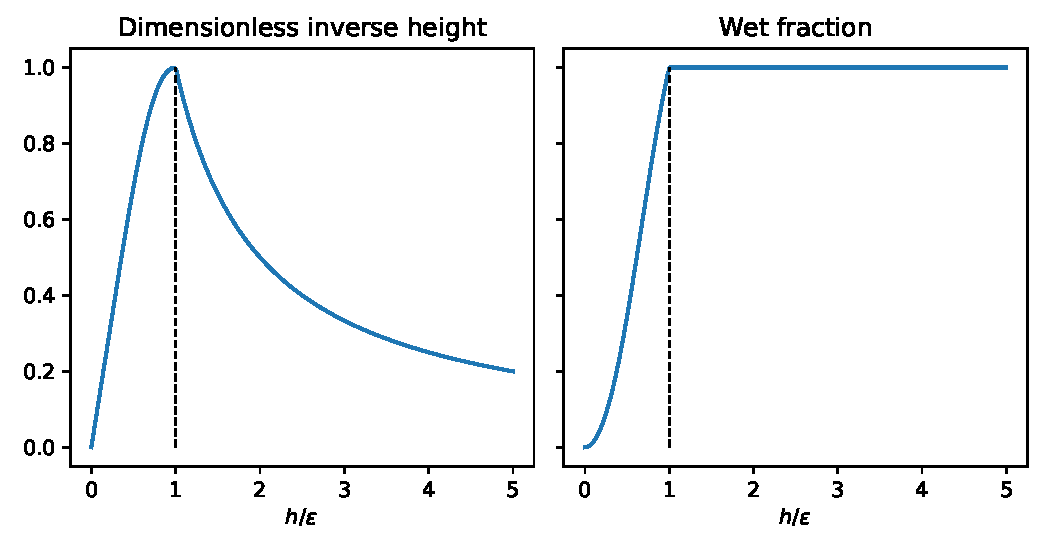
\includegraphics[width=\textwidth]{img/eulerian/inverse_height.pdf}
    \caption{Dimensionless functions to compute the  inverse height and the wet fraction.}
    \label{inverse_heihgt}
\end{figure}


% \paragraph{Partially wet elements}
% At the elements where the shoreline is located, the interpolated water depth will not represent the real water surface.
% Therefore, those elements need a special consideration in order to prevent unrealistic oscillations. Excluding those elements from the computations is equivalent to introduce an artificial barrier, and the inclusion of those elements will incur in a consideration of an extra volume of water.
% We chose to include all the elements in the computation and to modify the balance equations in order to satisfy equilibrium at rest (Figure \ref{partially_dry}). This is achieved by introducing a modified topography
% $z'$ which is obtained imposing the following equilibrium condition:
% \begin{equation}
%     \pder{\eta'}{x_i} = \pder{z'}{x_i} + \pder{h}{x_i} = \mathbf{0}
% \end{equation}

% \begin{figure}
%     \centering
%     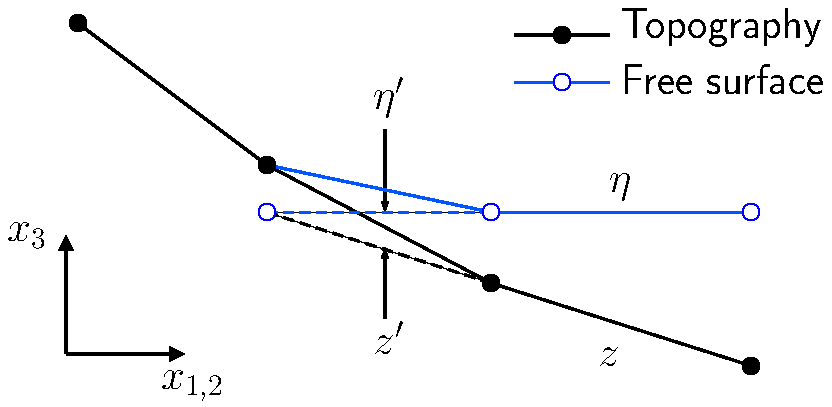
\includegraphics[width=.5\textwidth]{img/fig/partially_dry.pdf}
%     \caption{Dry, wet and partially wet elements in 1D. The dashed line shows the modified topography  and the corresponding free surface.}
%     \label{partially_dry}
% \end{figure}

% Following the idea of \cite{defina2000}, the identification of partially wet elements is done across the definition of a wet fraction function. In this research, instead of modifying the vertical integration of the Navier-Stokes equations, the wet fraction is  defined making use of the pseudo inverse $\hat{h}^{-1}$. The wet fraction $w$ reads:
% \begin{equation}
% w = h\hat{h}^{-1}
% \end{equation}

% The wet fraction function is defined in all the elements -wet, dry and partially dry- and its value goes from $0$ for dry elements to $1$ for wet elements (see Figure \ref{inverse_heihgt})
% This function makes possible to construct the source system vector $\mathbf{T}$ (see equations (\ref{discrete_sw}) and (\ref{discrete_sw_matrices})) with a linear combination between the two topographies as $wz + (1-w)z'$.


\paragraph{Avoiding the singularity of the system matrix}
Since all the elements are included in the computational domain, the last issue to overcome with small water depths are the numerical difficulties stated in Section \textcolor{red}{AAAAA}.
When there is a null water depth, the theoretical flow rate and velocity are zero. In that point the matrices $\mathbf{A}_i$ are not invertible and the eigenvalues are all equal to zero. In that case, the hyperbolicity property of the system is lost.
In practice, due to spurious oscillations, the flow rate and the velocity may be different from zero. The idea is to freeze the flow and to allow to invert the system matrix adding a diagonal of non zero terms to the momentum equation, i. e.,


\begin{equation}
\mathbf{G} \defeq \mathbf{G} + \xi\,\text{diag}(1, 1, 0)
\end{equation}


The selection of the areas where there is a dry domain is controlled with the wet fraction function and $\xi$ is defined as
\begin{equation}
\xi = k(1-w)
\end{equation}

In our numerical experiments we have chosen $k=10^3$.
The addition of a diagonal matrix remembers the artificial Manning friction proposed in \cite{heniche2000}. This term plays the role of freezing the flow in dry areas.


\paragraph{Mass conservation properties}
The stabilized method proposed is not monotonic and the dry domain model is acting to ensure stability, but it does not provide monotonicity. We note that all the modifications have been done at the momentum balance level. This means that mass is conserved globally by the weak formulation, but the mass sign preservation is not guaranteed.

Both unknowns, water depth and flow rate, are continuous at the dry-wet interface, but its derivatives are discontinuous. Even though the shock capturing scheme can not avoid this kind of oscillations, it will mitigate them, and the order of accuracy will be lost due to the introduction of the non-linear artificial diffusion \cite{badia2014}.






\subsection{Patch test}


Following Zienkiewicz \cite{zien1}, the patch test has been used as a first verification. The patch test is a basic verification which allows to verify the convergence. These tests have been developed imposing stationary solutions and obtaining the topography from the primary unknowns. The spatial domain $\Omega$ is a single element $e$.
Since the solution is stationary, the temporal domain is null and the test consist on the verification of zero accelerations.
Then, if the the solution belongs to the basis functions space, the test will pass analytically.
Otherwise, the test will pass asymptotically when the element is refined by subdivision of the domain ($h$-refinement). In that case, even if the element is not passing the test, the patch test is also useful since is checking the correctness of the implementation.

Several exact solutions have been applied to an element with size of $1m$. For the stabilized formulations a stabilization factor $\beta=0.01$ is used. The flux corrected solution depends directly on the stabilized formulation. If the solution belongs to the FE space, the obtained accelerations are less than $10^{-16}$, which is the round-off of machine precision.

\paragraph{Water at rest}
In this case, the free surface gradient and the velocity are zero. Some solutions can be built with that conditions, such as flat and non-flat topography, and bottom friction. In all the cases the accelerations are zero.

\paragraph{Slope in equilibrium}
This family of solutions verify constant water depth and constant velocity. The gravity terms (coming from the slope) are in equilibrium with the bottom friction terms. Several combinations are obtained with different directions of the slope and different Froude numbers, subcritical and supercritical.

\paragraph{Backwater analysis}
Finally, that family of analytical solutions, presents a constant flow rate where the gravity terms are in equilibrium with the bottom friction. But in that case, the primary unknowns do not belong to the FE space, since, either the velocity or the water depth are not linear. This test is passing asymptotically.


\subsection{Examples}
\label{sec:examples}

The FIC-FEM formulation presented has been implemented in KratosMultiphysics \cite{dadvand2010, dadvand2013}, an open source framework of numerical methods written in C++.
In this section we present four different examples. Three of them are oriented to verify a single aspect of the procedure explained in this research, the global stabilization, the shock capturing technique and the dry-wet interface.
The last one is devoted to test all the capabilities of the formulation in a practical case for which experimental data is available.


\subsubsection{Wave in a channel with a backward step}

The aim of the first example is to show that the Galerkin formulation applied to the shallow water equations is unstable and how the present stabilization method can overcome this issue. A calibration of the stabilization parameter is performed to optimize the effect of the stabilization terms in the obtained solution.
We study the propagation of a wave in a channel with a backward step (Figure \ref{step_mesh}) where all the boundaries are slip. The channel depth is 1m. An initial perturbation in the free surface at the left wall generates a wave which travels from 0 to 6s. The initial perturbation reads
\begin{equation}
\eta(t=0) = 0.05\cos(\pi x) \quad \text{if} \quad x<1, \quad \eta=0 \quad \text{otherwise}
\end{equation}


The wave is reflected at the right wall and then faces the step in the opposite direction.
Figure \ref{waves_propagation} shows the propagation of the wave along the channel.
The problem is discretized with a mesh fine enough to test the artificial diffusion added by the stabilization (Figure \ref{step_mesh}). The average element size is $0.06m$ and near the corner the mesh is refined to $0.02m$.
The time step is set automatically to keep a maximum Courant number equal to $1.0$ at every step. The problem is run three times with different algorithmic constants $\beta = 0.001$, $0.01$ and $0.1$. In this example, the shock capturing term is disabled.

\begin{figure}
    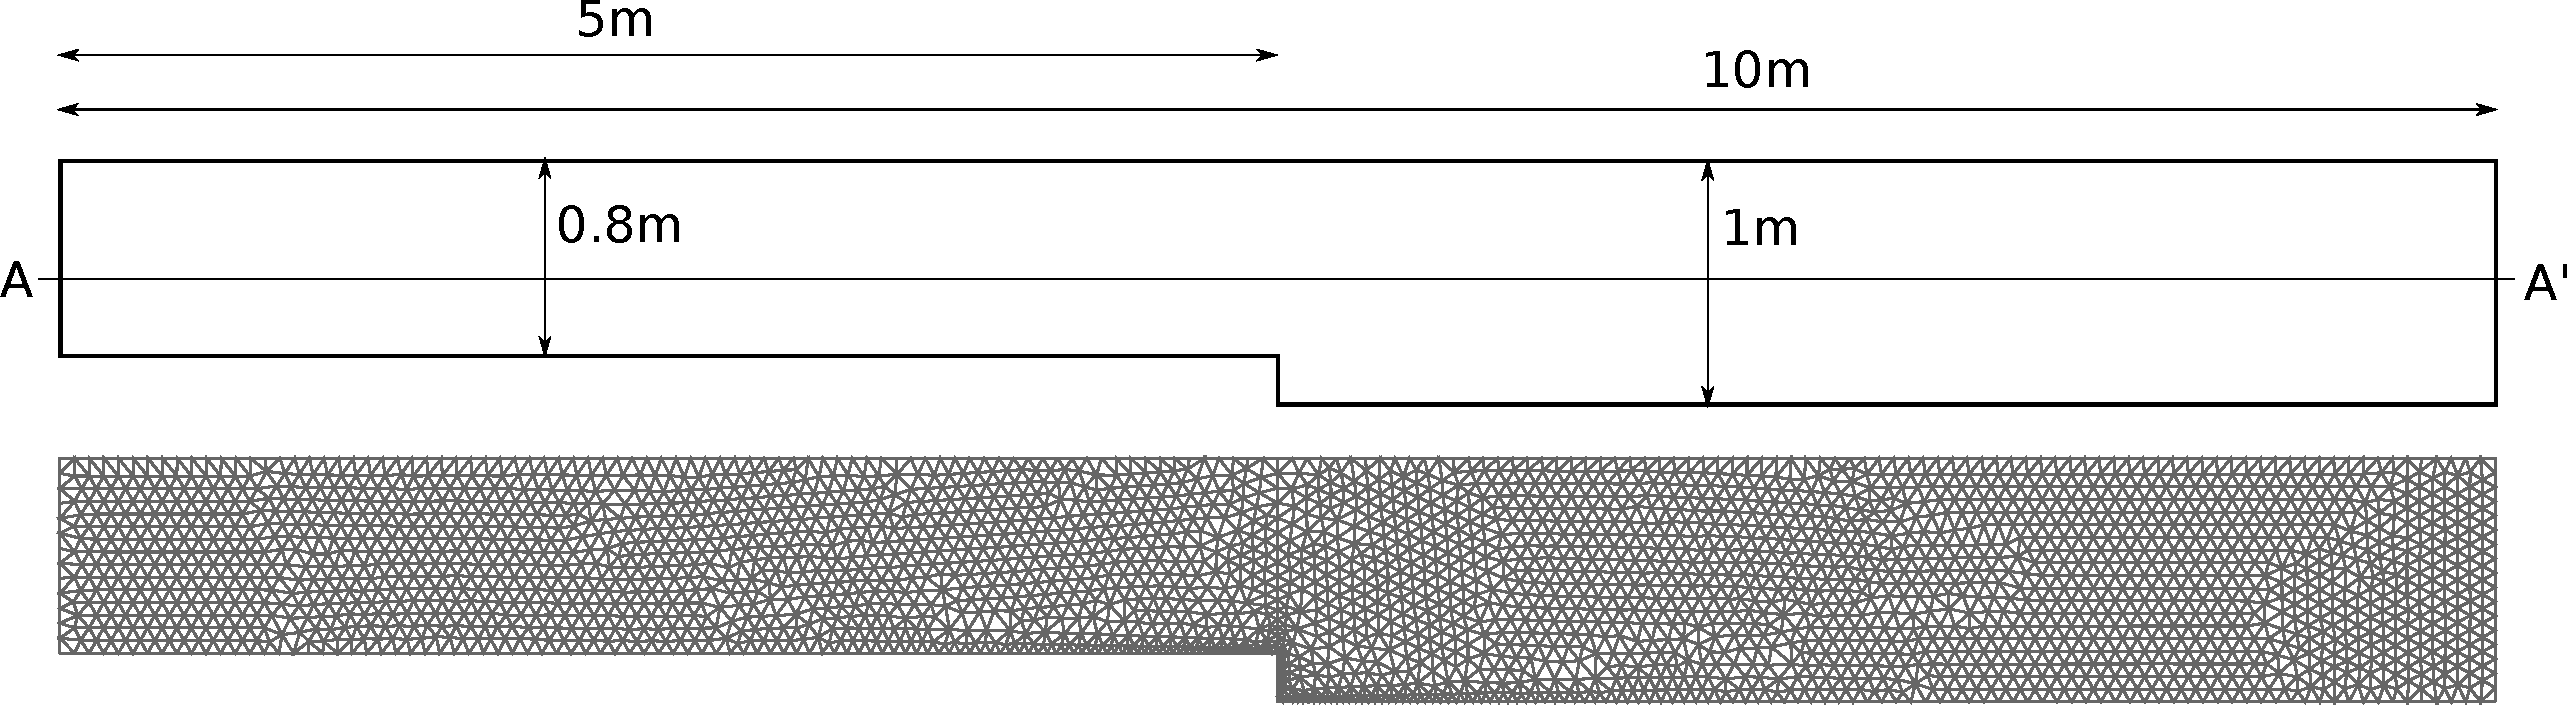
\includegraphics[width=\textwidth]{img/eulerian/step/geometry.pdf}
    \caption{Channel with a backward step. Domain and mesh used in the simulation. All the boundary conditions are slip. The average element size is $0.06m$. Near the obstacle the mesh size is $0.02m$. There are $3.125$ nodes and $5.826$ elements.}
    \label{step_mesh}
\end{figure}

\begin{figure}[H]
\begin{subfigure}{\textwidth}
    \centering
    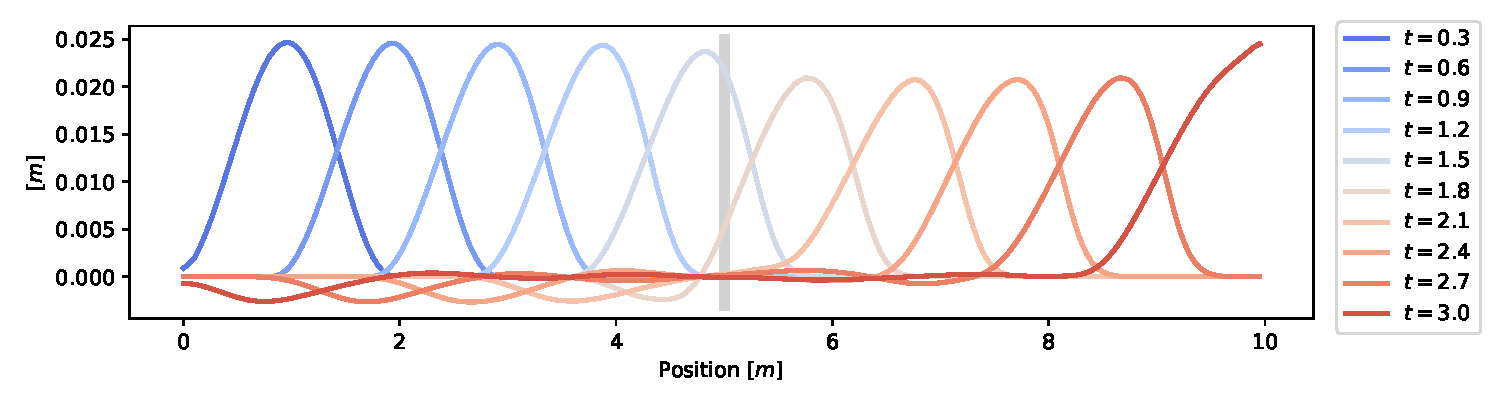
\includegraphics[width=\textwidth]{img/eulerian/step/free_surface_1.pdf}
    \caption{Time from $0$ to $3s$}
\end{subfigure}
\begin{subfigure}{\textwidth}
    \centering
    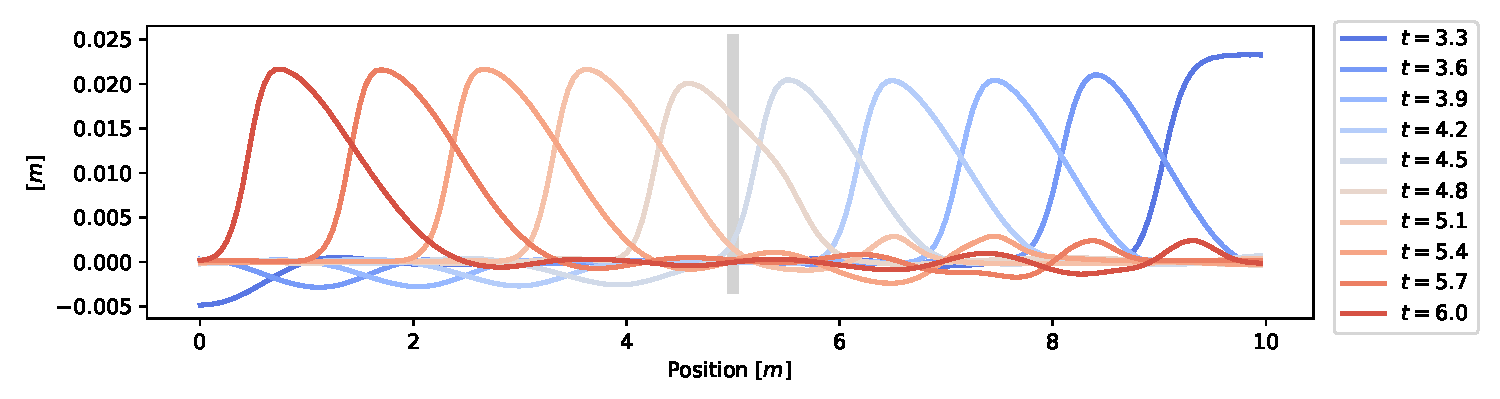
\includegraphics[width=\textwidth]{img/eulerian/step/free_surface_2.pdf}
    \caption{Time from $3$ to $6s$}
\end{subfigure}
\caption{Channel with a backward step. Timestamps of the free surface along the cut AA' from Figure \ref{step_mesh}. (a) The initial perturbation is propagating to the right. (b) Propagation of the reflected wave from right to left.}
\label{waves_propagation}
\end{figure}


The best results are achieved with the intermediate value and it has been fixed for the rest of the examples in this paper.
Figures \ref{stab_parameters_time1} and \ref{stab_parameters_time2} show that the lower value of $\beta$ is not enough to provide stability, while the higher value is over diffusive.

\begin{figure}[H]
\begin{subfigure}{.05\textwidth}
    \caption{}
\end{subfigure}
\begin{minipage}[c]{.94\textwidth}
    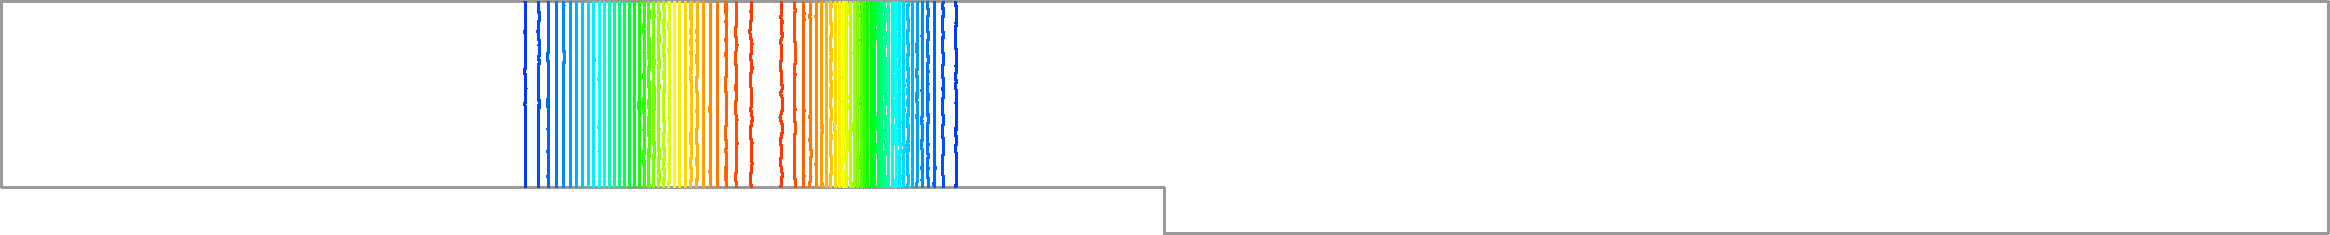
\includegraphics[width=\textwidth]{img/eulerian/step/stab_0.001_time_1.pdf}        
\end{minipage}
\par\medskip
\begin{subfigure}{.05\textwidth}
    \caption{}
\end{subfigure}
\begin{minipage}[c]{.94\textwidth}
    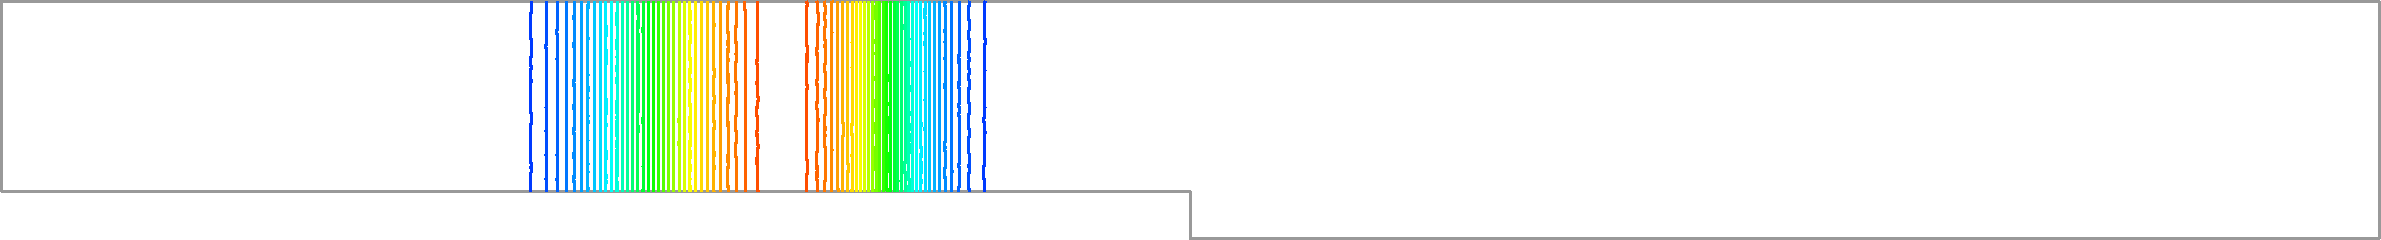
\includegraphics[width=\textwidth]{img/eulerian/step/stab_0.01_time_1.pdf}        
\end{minipage}
\par\medskip
\begin{subfigure}{.05\textwidth}
    \caption{}
\end{subfigure}
\begin{minipage}[c]{.94\textwidth}
    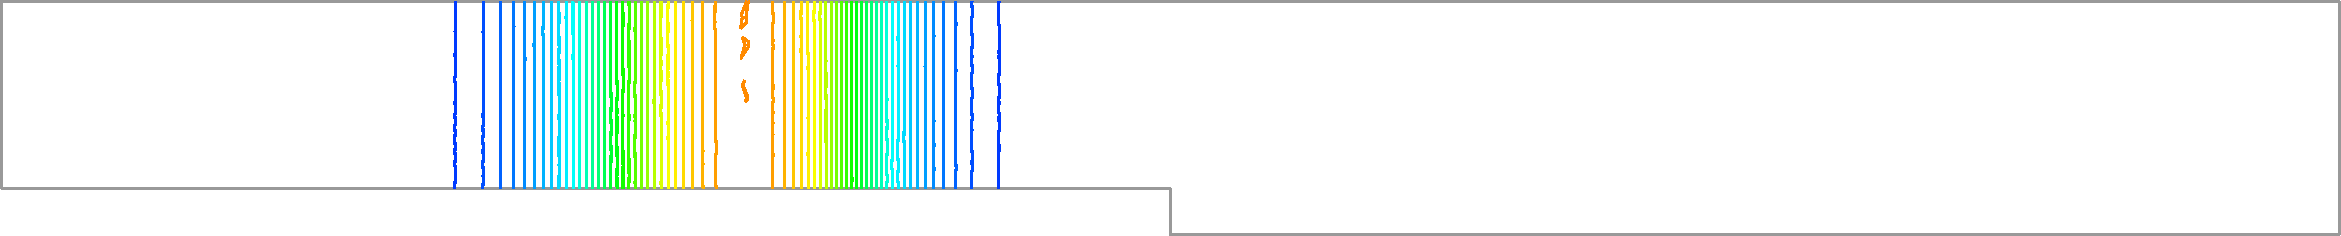
\includegraphics[width=\textwidth]{img/eulerian/step/stab_0.1_time_1.pdf}        
\end{minipage}
\caption{Channel with a backward step. Contour plots of the free surface elevation at time $t=1s$ for different stabilization factors. (a) $\beta=0.001$, (b) $\beta=0.01$, (c) $\beta=0.1$}
\label{stab_parameters_time1}
\end{figure}

\begin{figure}[H]
    \begin{subfigure}{.05\textwidth}
        \caption{}
    \end{subfigure}
    \begin{minipage}[c]{.94\textwidth}
        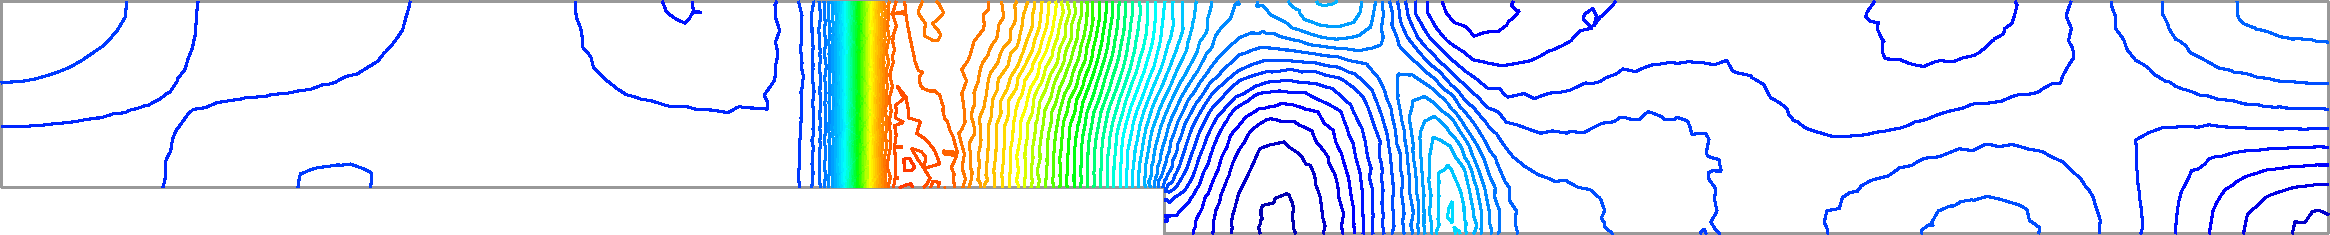
\includegraphics[width=\textwidth]{img/eulerian/step/stab_0.001_time_5.pdf}
    \end{minipage}
    \par\medskip
    \begin{subfigure}{.05\textwidth}
        \caption{}
    \end{subfigure}
    \begin{minipage}[c]{.94\textwidth}
        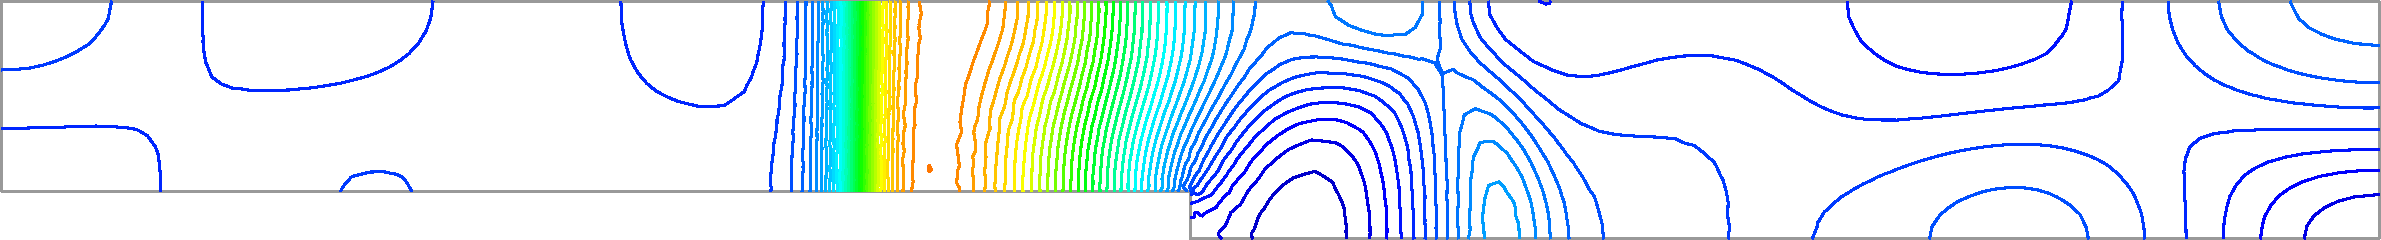
\includegraphics[width=\textwidth]{img/eulerian/step/stab_0.01_time_5.pdf}
    \end{minipage}
    \par\medskip
    \begin{subfigure}{.05\textwidth}
        \caption{}
    \end{subfigure}
    \begin{minipage}[c]{.94\textwidth}
        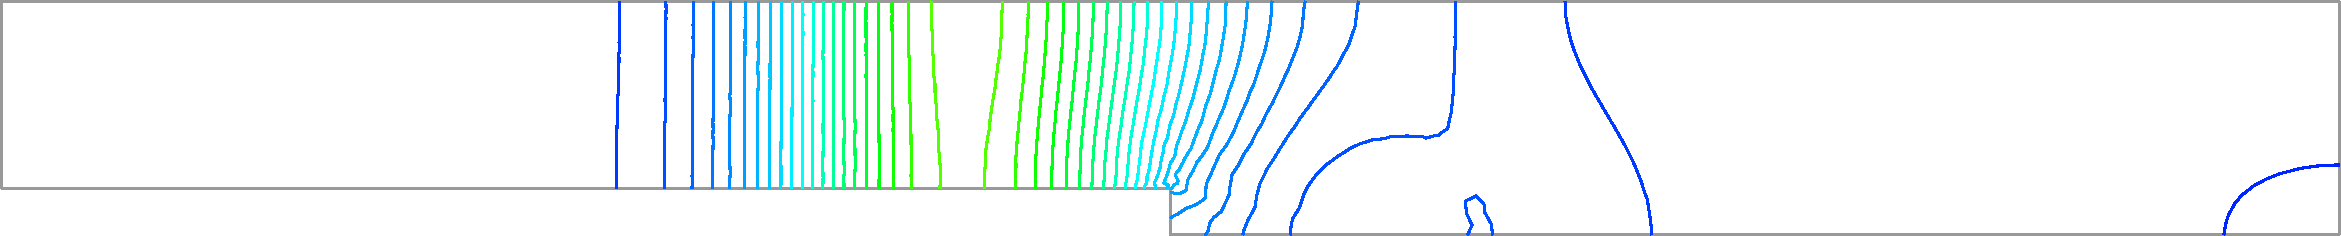
\includegraphics[width=\textwidth]{img/eulerian/step/stab_0.1_time_5.pdf}
    \end{minipage}
\caption{Channel with a backward step. Contour plots of the free surface elevation at time $t=5s$ for different stabilization factors. (a) $\beta=0.001$, (b) $\beta=0.01$, (c) $\beta=0.1$}
\label{stab_parameters_time2}
\end{figure}



\subsubsection{Oscillation in a parabolic basin}

The second example is a classical benchmark oriented to test the accuracy of the location of the moving boundary. The topography follows a parabolic profile while the initial free surface elevation is planar and intersects the topography. The initial configuration corresponds to zero velocity but the free surface is in a non horizontal plane. The solution of the problem is oscillatory and the free surface elevation remains planar. An analytical solution can be found in the compilation made by Delestre et al. \cite{delestre2013}.

The domain $\Omega$ is defined in the interval $[0,L]\times[0,1]m$ where $L=10m$ and all the boundaries are reflective ($\mathbf{u}\cdot\mathbf{n} = 0$). The topography is given by the following expression
\begin{equation}
z(x,y) = h_0 \left(\frac{1}{a^2}\left(x - \frac{L}{2}\right)^2 - 1\right)
\end{equation}
The primitive variables are defined by
\begin{subequations}
\begin{align}
h(x,y) &=
\begin{cases}
-h_0\left(\left(\frac{1}{a}\left(x - \frac{L}{2}\right) + \frac{1}{2a}\cos(2Bt)\right)^2 - 1\right)
\quad &\text{if} \ x_1(t) < x < x_2(t) \\
0 \quad &\text{otherwise}
\end{cases} \\
\mathbf{u}(x,y) &=
\begin{cases}
(B,0)\sin(2Bt) \quad &\text{if} \ x_1(t) < x < x_2(t) \\
(0,0) \quad &\text{otherwise}
\end{cases}
\end{align}
\end{subequations}
where $B=\sqrt{2gh_0}/2a$, and $x_1$, $x_2$ are time dependent functions which define the location of the dry-wet interface:
\begin{equation}
\begin{split}
x_1(t) = -\frac{1}{2}\cos(2Bt) - a + \frac{L}{2} \\
x_2(t) = -\frac{1}{2}\cos(2Bt) + a + \frac{L}{2}
\end{split}
\end{equation}

In that example the selected parameters are $h_0=1m$ and $a=1m$.

The domain $\Omega$ is discretized using several meshes in order to perform a convergence analysis. The meshes employed are listed in Table \ref{parabola_convergence}. Figure \ref{parabola_mesh} shows one of the intermediate mesh. Once the simulation begins, the water starts to oscillate on the parabolic basin and the velocity field is constant on the spatial domain, while follows a periodic function respect to the time.

\begin{figure}
    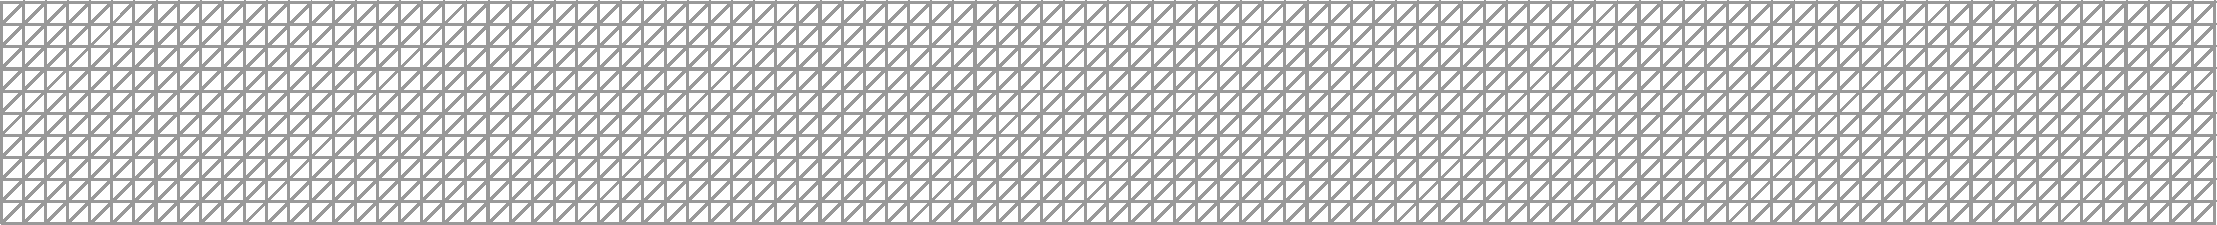
\includegraphics[width=\textwidth]{img/eulerian/par/mesh_0.1.pdf}
    \caption{Parabolic basin. One of the meshes used in the analysis. The element size is $0.1m$.}
    \label{parabola_mesh}
\end{figure}

Figure \ref{parabola_graphic} shows a cut along the mesh at different times. The most challenging problem is to capture the discontinuity of the velocity. Even though the velocity presents a discontinuity, it isn't the origin of the oscillatory behavior since the velocity is not a degree of freedom. It can be appreciated how the discontinuity of the velocity is not an issue.

\begin{figure}
\begin{subfigure}{0.4\textwidth}
    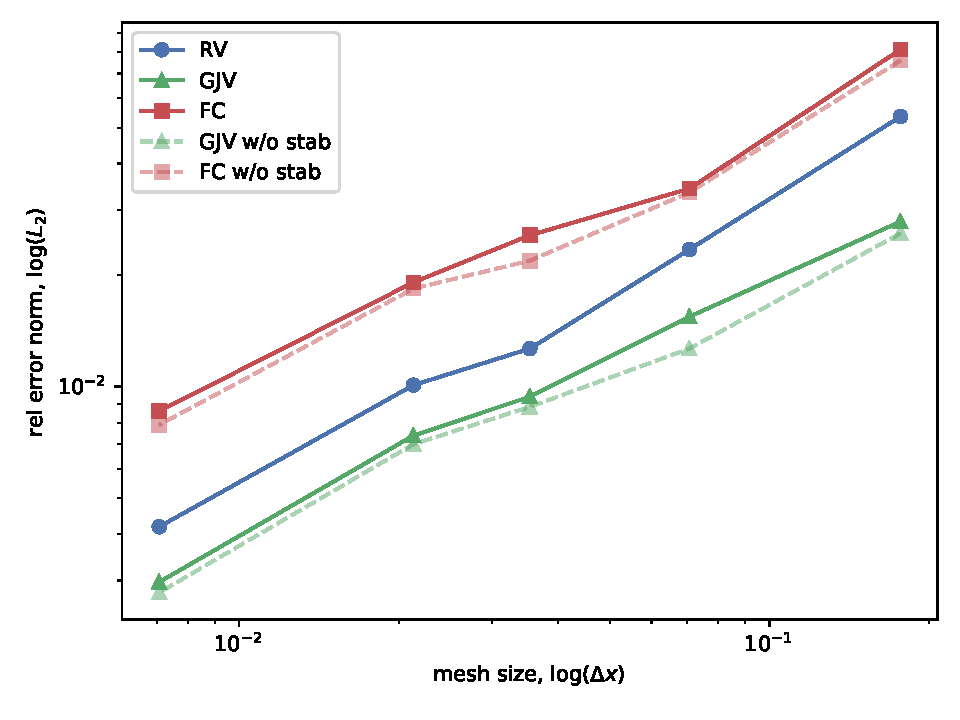
\includegraphics[width=\textwidth]{img/eulerian/par/conv_1.pdf}    
\end{subfigure}
\hfill
\begin{subfigure}{0.58\textwidth}
    \begin{tabular}{>{\small}rcccc} \hline
    $n_{nodes}$ & $\Delta x$ & $\Delta t$ & CFL & $L_2(e_{rel})$ \\ \hline
205 & 0.25 & 0.008 & 0.5 & 0.24 \\
1,111 & 0.1 & 0.003 & 0.5 & 0.064 \\
4,221 & 0.05 & 0.002 & 0.5 & 0.023 \\
11,356 & 0.03 & 0.001 & 0.5 & 0.013 \\
101,101 & 0.01 & 0.0003 & 0.5 & 0.0049 \\
    \hline
    \end{tabular}
\end{subfigure}
\caption{Parabolic basin. Convergence analysis for the water height.}
\label{parabola_convergence}
\end{figure}

\begin{figure}[H]
\begin{subfigure}{\textwidth}
    \centering
    Time $t=0.5s$
    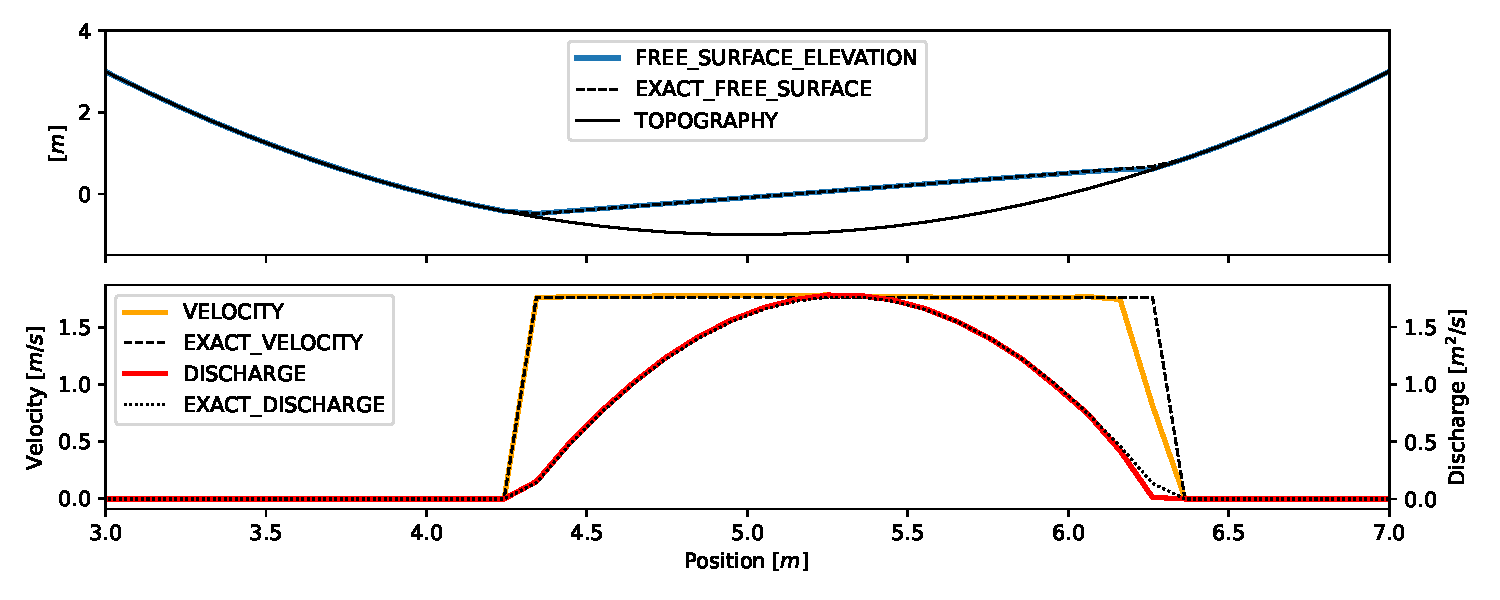
\includegraphics[width=\textwidth]{img/eulerian/par/parabola_t0.5.pdf}
\end{subfigure}
\par\medskip
\begin{subfigure}{\textwidth}
    \centering
    Time $t=1s$
    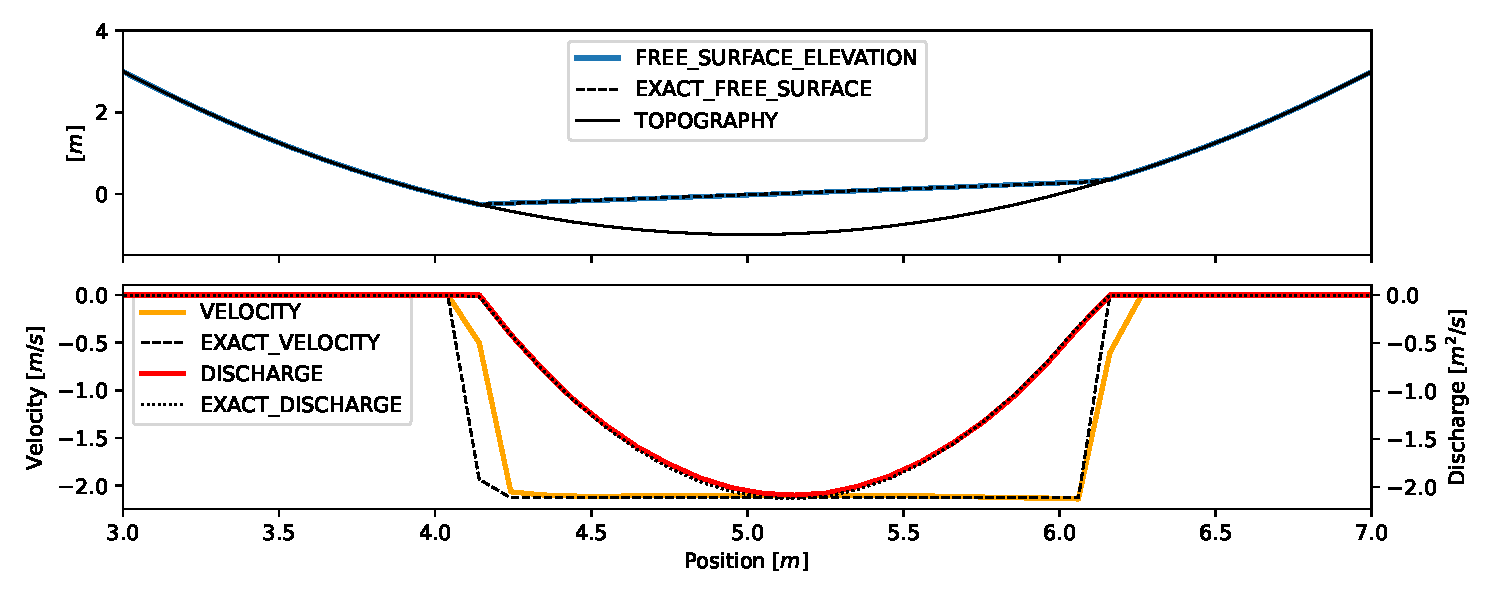
\includegraphics[width=\textwidth]{img/eulerian/par/parabola_t1.0.pdf}
\end{subfigure}
\caption{Parabolic basin. Cuts along the mesh of size $0.03m$ at different times. There are 333 nodes on the cut.}
\label{parabola_graphic}
\end{figure}

A mass conservation test is performed with the mesh of size $0.05m$ in a simulation of $5s$. The results are presented in Figure \ref{parabola_mass}. The integration of the mass is performed over all the domain and over the wet domain. The wet domain is identified with the wet fraction, requiring that it is equal to $1$. Since the presented scheme is not mass sign preserving, the wet mass can not be equal to the total mass and a small fraction is lost from the wet domain. The loss depends on the element size and presents an oscillatory behavior inherent of the method. Figure \ref{parabola_mass} shows that the mass loss is bounded and the mean does not increase with time.


\begin{figure}[H]
    \centering
    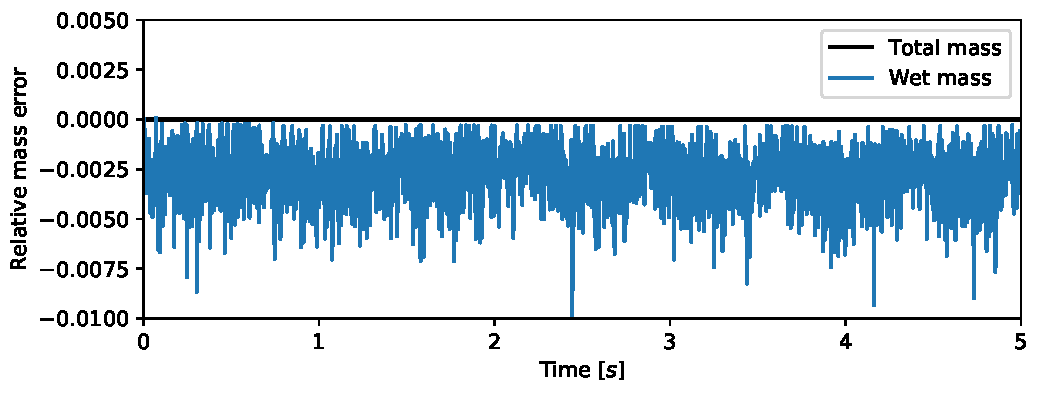
\includegraphics[width=.95\textwidth]{img/eulerian/par/mass_conservation}
    \caption{Parabolic basin. Mass conservation error. The element size used in this simulation is $0.05m$.}
    \label{parabola_mass}
\end{figure}

Figure \ref{parabola_results} shows the results using the finest mesh. The discretization is not shown for the sake of simplicity. As expected, there is no variation on the results in the transversal section.

\begin{figure}[H]
    \begin{subfigure}{.05\textwidth}
        \caption{}
    \end{subfigure}
    \begin{minipage}[c]{.94\textwidth}
        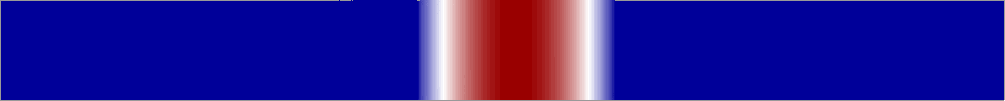
\includegraphics[width=\textwidth]{img/eulerian/par/height_1.0.png}
    \end{minipage}
\par\medskip
    \begin{subfigure}{.05\textwidth}
        \caption{}
    \end{subfigure}
    \begin{minipage}[c]{.94\textwidth}
        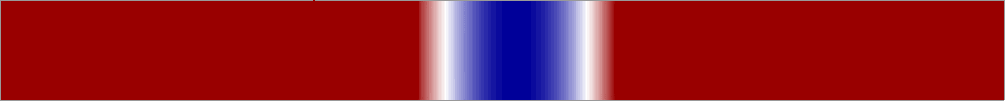
\includegraphics[width=\textwidth]{img/eulerian/par/momentum_1.0.png}
    \end{minipage}
\par\medskip
    \begin{subfigure}{.05\textwidth}
        \caption{}
    \end{subfigure}
    \begin{minipage}[c]{.94\textwidth}
        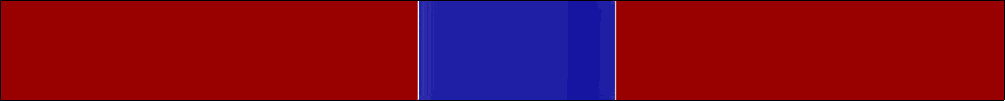
\includegraphics[width=\textwidth]{img/eulerian/par/velocity_1.0.png}
    \end{minipage}
\caption{Parabolic basin. Results with the fine mesh of size $0.01m$ at time $t=1s$. (a) Water height, (b) x-discharge and (c) x-velocity. There is no legend for simplicity, the red colour is positive and blue means a null or negative magnitude.}
\label{parabola_results}
\end{figure}



\subsubsection{Short channel with smooth transition and shock}

The third example in a benchmark based on the Mac Donald's type solutions \cite{macdonald1997}. The analytical solution can be found in the same compilation than the previous example \cite{delestre2013}. This test presents a channel with a steady state solution. There is a subcritical inlet and a transcritical flow is produced. The outlet is also subcritical and then a shock is generated at $\sfrac{2}{3}$ of the channel. The aim of this example is to evaluate the shock capturing technique presented and the correct location of the hydraulic jump, which depends on the bottom friction law.

Here we will consider the 1D shallow water equations without diffusion and only with Manning bottom friction as source term. A steady state solution satisfies $\pder{q}{x}=0$ and Equation (\ref{general_sw}) reduces to
\begin{equation} \label{steady_state}
\pder{z}{x} = \left(\frac{v^2}{gh}-1\right) \pder{h}{x} - n^2\frac{\abs{v}v}{h^{\sfrac{4}{3}}}
\end{equation}
This relation allows to integrate the topography given an analytical expression for the water height. Another approach in hydraulics is to consider a given discharge and topography and integrate the water height using Equation (\ref{steady_state}). Following both approaches exact solutions can be obtained. Since this expression involves the bottom friction, we can verify if the friction term is correctly coded in order to satisfy the steady state.

For this benchmark we have considered the domain defined by the spatial domain $[0,100]\times[0,5]$ which is a channel of $100m$ length and $5m$ width (Figure \ref{chanel_geometry}), and the following boundary conditions:
\begin{equation}
\begin{split}
    q_x = 2\ \text{m/s} \quad &\text{in} \quad \Gamma_{upstream} \\
    h = h_{ex}(100) \quad &\text{in} \quad \Gamma_{downstream} \\
    q_y = 0 \quad &\text{in} \quad \Gamma_{walls}
\end{split}
\end{equation}

The problem is initialized with the following values:
\begin{equation}
\begin{split}
    h(x,0) &= \max(h_{ex}(100) - z(x), h_{ex}(0)) \\
    \mathbf{q}(x,0) &= \mathbf{0}
\end{split}
\end{equation}

The Manning coefficient is $0.0328\ \text{m}^{-1/3}\text{s}$ and the water height $h_{ex}(x)$ is a piecewise function defined in \cite{delestre2013}. The discontinuity of the water height function is located at $x=200/3m$ and defines the hydraulic jump. The expression of the stationary exact water depth is:
\begin{equation} \label{jump_height_definition}
    h_{ex} = \begin{cases}
        \left(\frac{4}{g}\right)^\frac{1}{3} \left(\frac{4}{3} - \frac{x}{L}\right) - \frac{9x}{10L}
            \left(\frac{x}{L} - \frac{2}{3}\right) \, ,\ \text{for} \ x < \frac{2L}{3}\\
        \left(\frac{4}{g}\right)^\frac{1}{3} \left(
              a_1 \left(\frac{x}{L} - \frac{2}{3}\right)^4
            + a_1 \left(\frac{x}{L} - \frac{2}{3}\right)^3
            - a_2 \left(\frac{x}{L} - \frac{2}{3}\right)^2 \right. \\ \left. \qquad\qquad\qquad\qquad
            + a_3 \left(\frac{x}{L} - \frac{2}{3}\right)
            + a_4
        \right) \, ,\ \text{for} \ x \geq \frac{2L}{3}
    \end{cases}
\end{equation}
where $a_1=0.674202m$, $a_2=21.7112m$, $a_3=14.492m$, $a_4=1.4305m$ and $L=100m$. The topography is obtained by a numerical integration using the fourth order Runge Kutta method.

As in the previous example, several meshes are employed and a convergence analysis is performed (Figure \ref{hydraulic_jump_convergence}). The shock capturing parameter is $\alpha=1.0$ and we will study the accuracy of the hydraulic jump. 
Given the initial conditions, the hydraulic jump is generated between the first $50$ and $80s$. The overall error is computed at time $t=200s$, in order to ensure the stationary state is achieved.
The table from Figure \ref{hydraulic_jump_convergence} shows the error of the $x$-discharge over all the domain using the $L_2$ norm.

Results from different meshes are compared in Figures \ref{mac_donald_shock_graph_5} and \ref{mac_donald_shock_graph_2}. The oscillations are reduced with the finer mesh (Figure \ref{mac_donald_shock_graph_2}), but there is a peak on the discharge at the location of the shock. This peak is initiated because the momentum balance includes the gradient of the total water depth, and the analytical gradient is a Dirac delta function.

\begin{figure}
    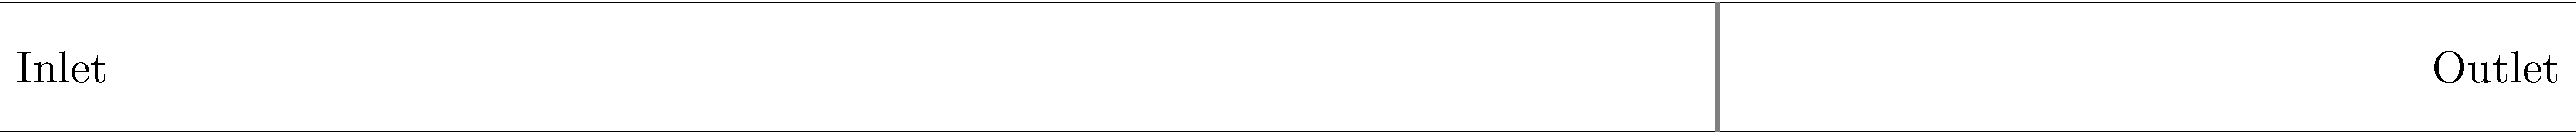
\includegraphics[width=\textwidth]{img/eulerian/jump/sketch.pdf}
    \caption{Short channel. Geometry of the channel. The vertical line shows the position of the hydraulic jump.}
    \label{chanel_geometry}
\end{figure}


\begin{figure}
\begin{subfigure}{0.4\textwidth}
    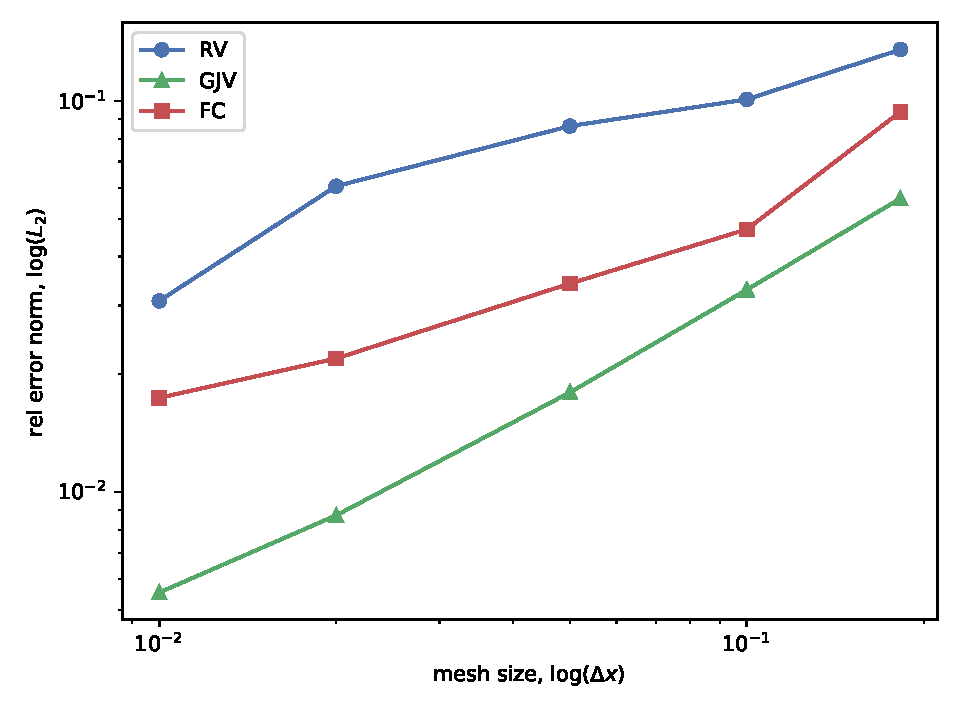
\includegraphics[width=\textwidth]{img/eulerian/jump/momentum_convergence.pdf}    
\end{subfigure}
\hfill
\begin{subfigure}{0.58\textwidth}
    \begin{tabular}{>{\small}rcccc} \hline
    $n_{nodes}$ & $\Delta x$ & $\Delta t$ & CFL   & $L_2(e_{rel})$ \\ \hline
    204         &        2.0 &      0.005 & 0.016 & 0.177 \\
    606         &        1.0 &      0.005 & 0.031 & 0.138 \\
    2211        &        0.5 &      0.005 & 0.062 & 0.088 \\
    13026       &        0.2 &      0.005 & 0.15  & 0.041 \\ \hline
    \end{tabular}
\end{subfigure}
\caption{Short channel. Convergence analysis for the $x$-discharge.}
\label{hydraulic_jump_convergence}
\end{figure}


\begin{figure}
    \centering
    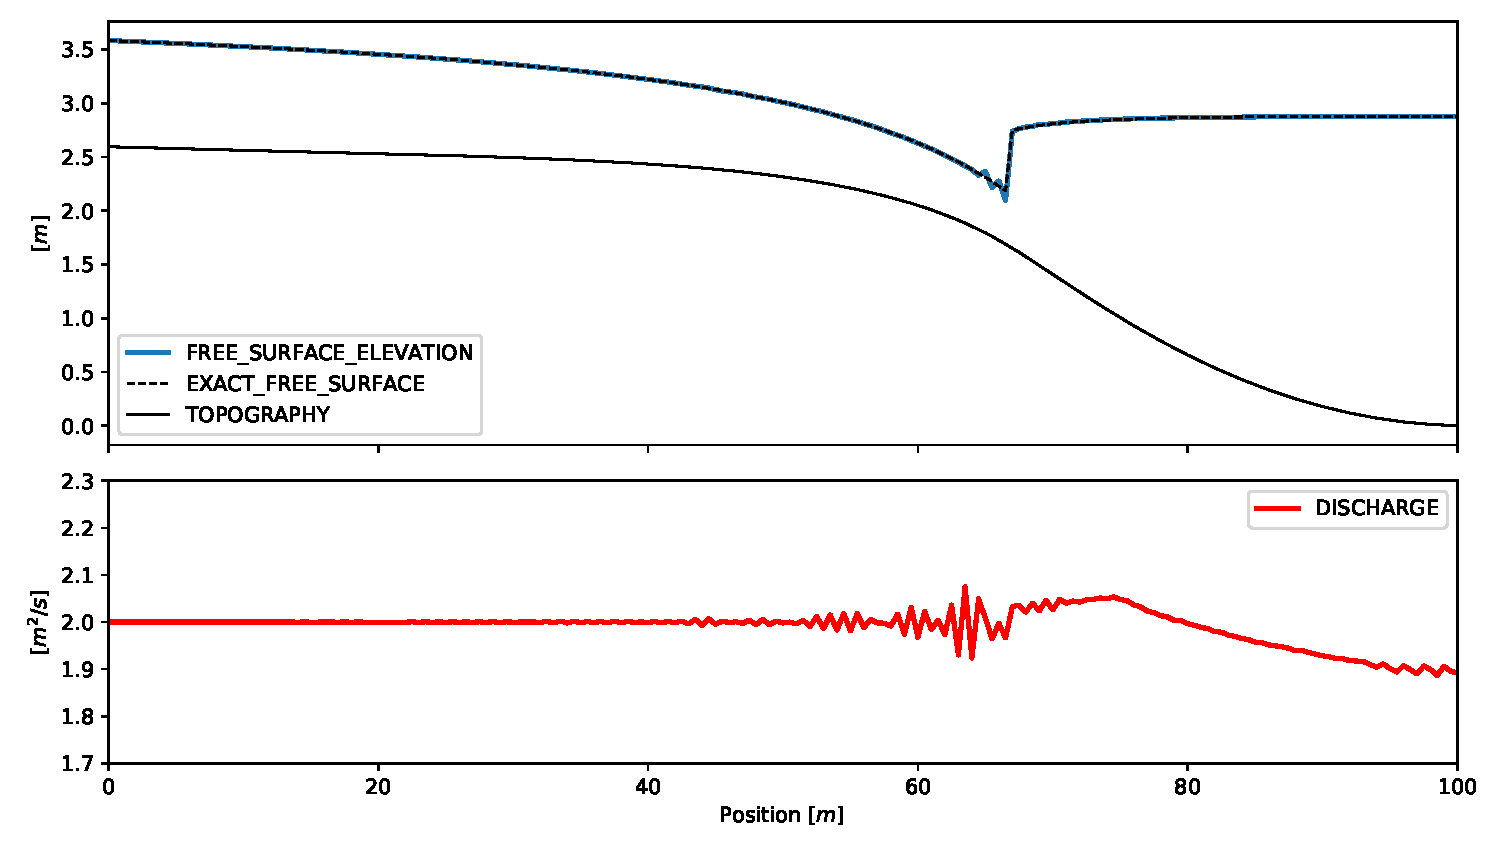
\includegraphics[width=\textwidth]{img/eulerian/jump/mesh_0.5.pdf}
    \caption{Short channel. Graph along the cut defined by the center of the channel. The mesh size is $0.5m$}
    \label{mac_donald_shock_graph_5}
\end{figure}

\begin{figure}
    \centering
    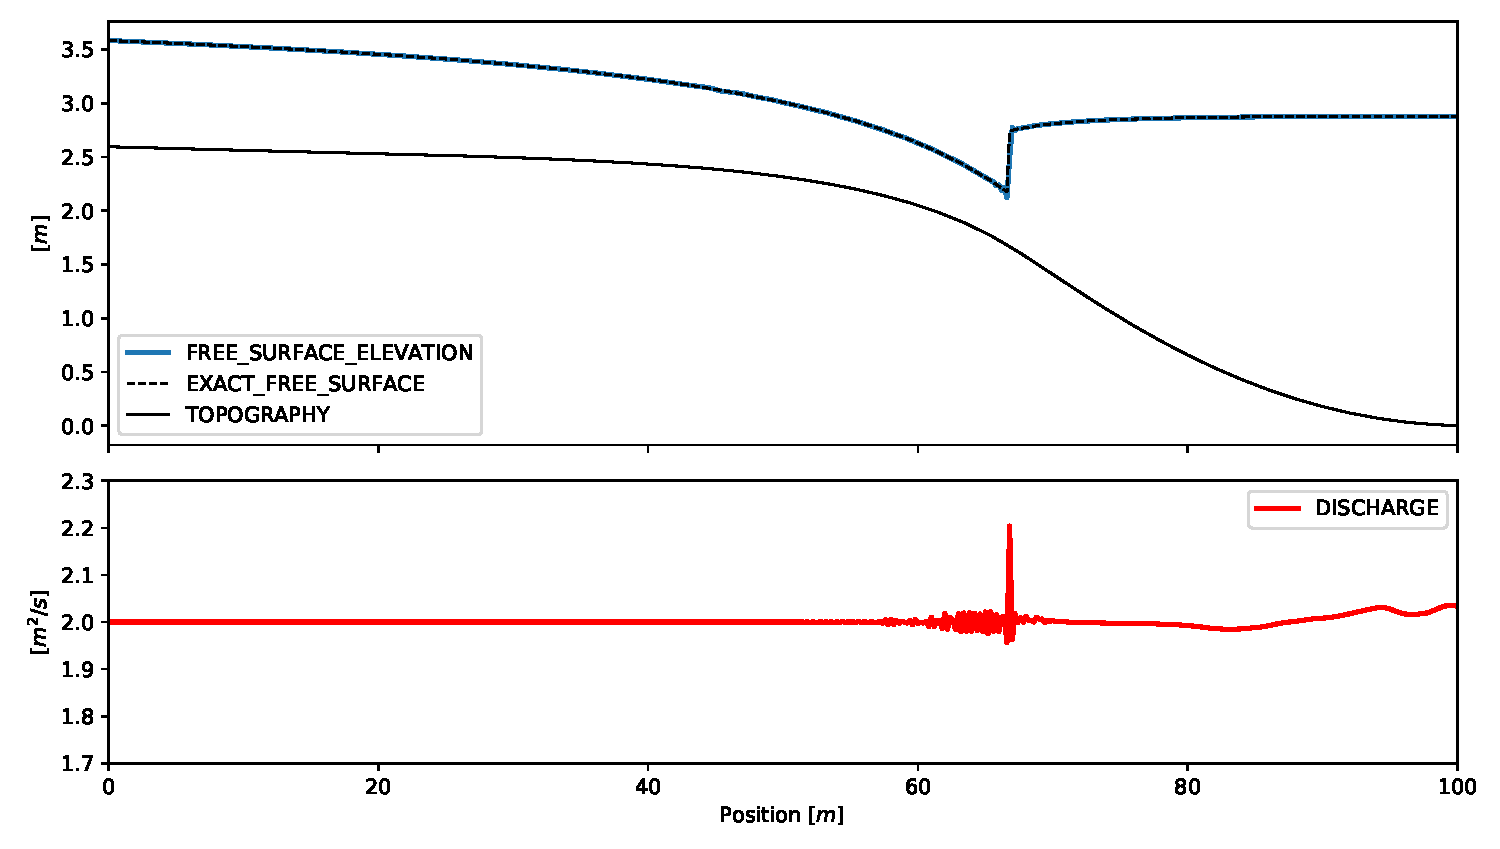
\includegraphics[width=\textwidth]{img/eulerian/jump/mesh_0.2.pdf}
    \caption{Short channel. Graph along the cut defined by the center of the channel. The mesh size is $0.2m$}
    \label{mac_donald_shock_graph_2}
\end{figure}


\subsubsection{Experimental dam break flow against an isolated building}

The last example consists on the reproduction of the experiment carried out by Soares \cite{soares2007}.
A dam break flow with a building downstream is simulated. The problem definition is depicted in Figure \ref{experiment_sketch}. The channel is $3.4m$ wide and the end of the dam is located at $x=0$.
As initial conditions, the water depth is set to $0.4m$ in the reservoir, while the channel is dry. The Manning coefficient is $0.01sm^{-\sfrac{1}{3}}$ over all the domain.
At the beginning of the simulation, the gate of the dam is removed and the water is allowed to flow around the building.

There are some gauges (Table \ref{gauges_positions} and Figure \ref{experiment_sketch}) where the water height and velocity are recorded. Experimental data is used to validate the numerical method.

\begin{figure}[H]
\centering
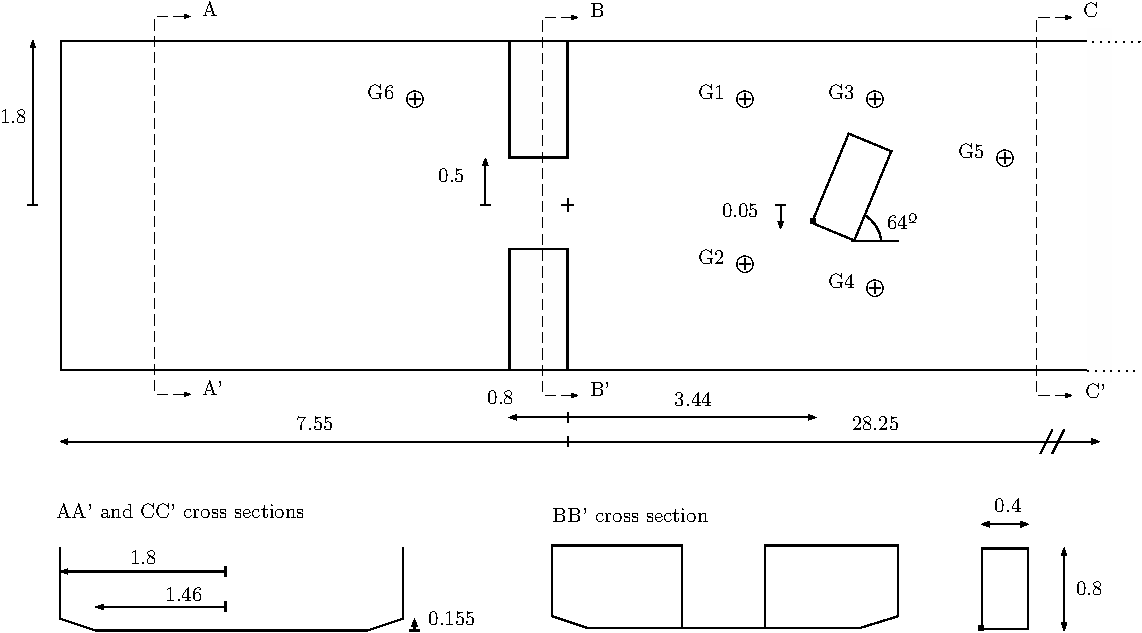
\includegraphics[width=\textwidth]{img/eulerian/exp/sketch.pdf}
\caption{Experimental dam break flow. Definition of the isolated building benchmark. The dimensions are in $m$.}
\label{experiment_sketch}
\end{figure}

\begin{table}
\centering
\begin{tabular}{ccc}
\hline
Gauge number & X & Y \\ \hline
1 &  2.65 &  1.15 \\
2 &  2.65 & -0.60 \\
3 &  4.00 &  1.15 \\
4 &  4.00 & -0.80 \\
5 &  5.20 &  0.30 \\
6 & -1.87 &  1.10 \\ \hline
\end{tabular}
\caption{Experimental dam break flow. Positions of the gauges, units in $m$.}
\label{gauges_positions}
\end{table}

The domain is discretized with a mesh with an average element size of $0.05m$. There are 115.000 elements and the time step is computed to keep a courant number of 1.0. Figure \ref{experiment_mesh} displays two details of the mesh, near the dam and around the building.

\begin{figure}[H]
\centering
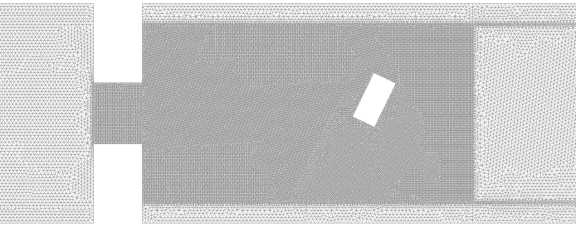
\includegraphics[width=.8\textwidth]{img/eulerian/exp/experiment_mesh.png}
\caption{Experimental dam break flow. Detail of the mesh near the dam and around the building. The coarse elements have an average size of $0.06m$ and the refined area has an average element size of $0.02m$. There are 160.000 elements.}
\label{experiment_mesh}
\end{figure}

To get a general idea of the flow, Figure \ref{experiment_plots} shows several results of the water depth after the gate release. Figure \ref{experiment_gauges} shows the evolution of the water depth at the gauges. An initial delay is observed in the propagation of the front in the gauges 1 to 5.

\begin{figure}
\centering
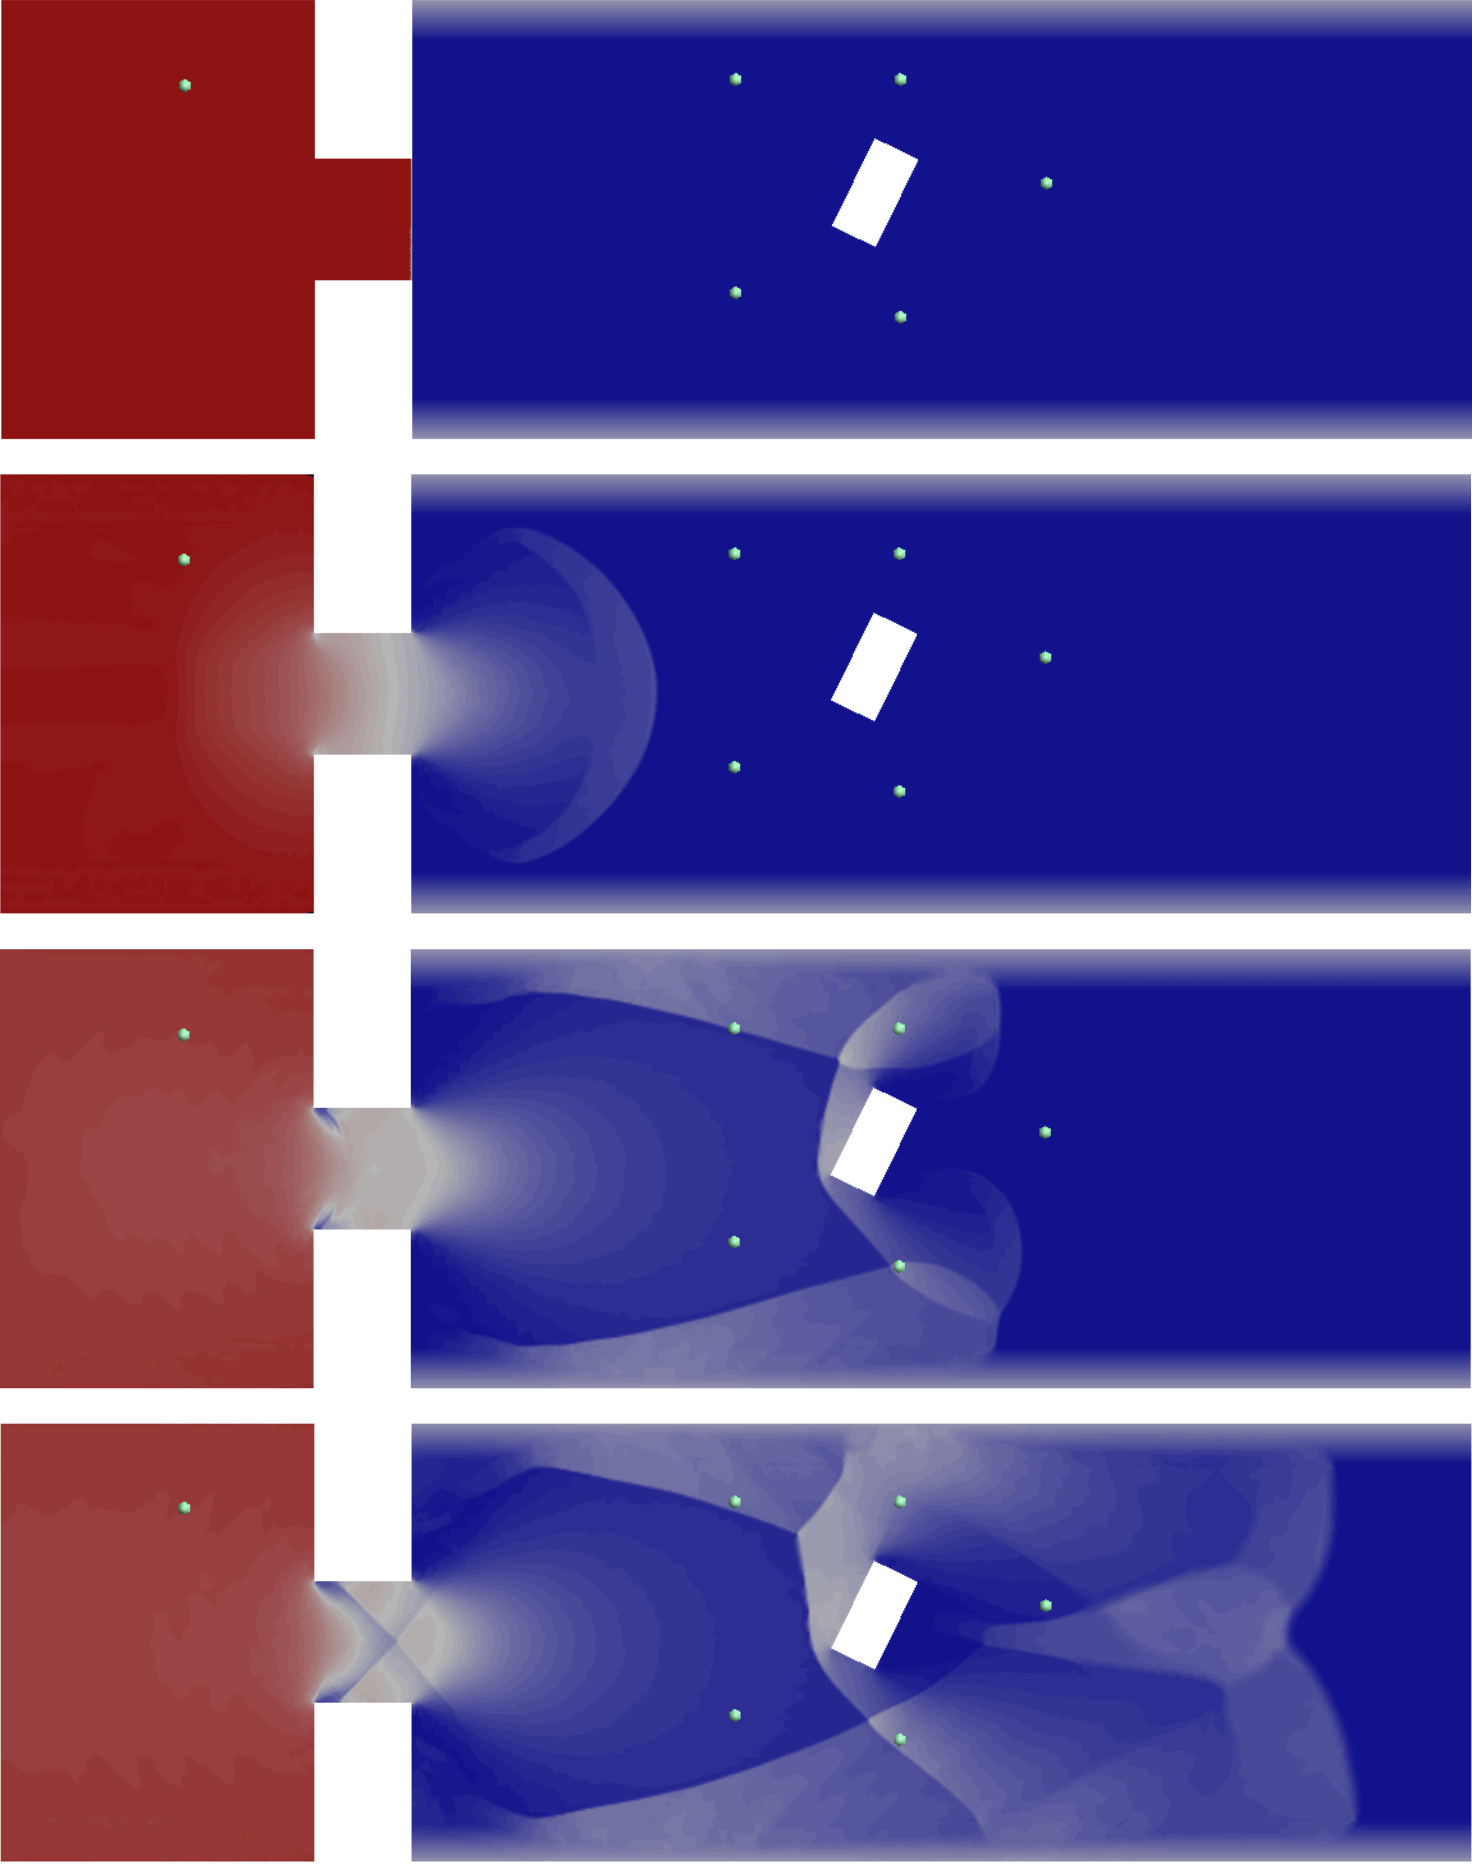
\includegraphics[width=\textwidth]{img/eulerian/exp/results.png}
\caption{Experimental dam break flow. Results of the benchmark at times $0$, $1$ and $3$ seconds}
\label{experiment_plots}
\end{figure}


Gauge 1 is located upstream of the building and close to the left wall of the channel. In gauge 1 there are the main discrepancies between the numerical and experimental results. The vicinity of the wall is responsible for the rapid variations in the water level. After the arrival of the front wave, this is reflected in the wall and a second raise of the water level is observed. About $t=6s$, an oblique hydraulic jump is formed and registered in gauge 1. The two first shocks are well captured by the numerical results, but the oblique hydraulic jump is registered latter, at $t=10s$, and there is a general overestimation of the ones for the water depth values.

The main hydraulic jump in gauge 2 formed by the reflection against the building is registered at $t=15s$, but in the numerical simulation is it formed very rapidly, presenting a discontinuity in time.

\begin{figure}
\centering
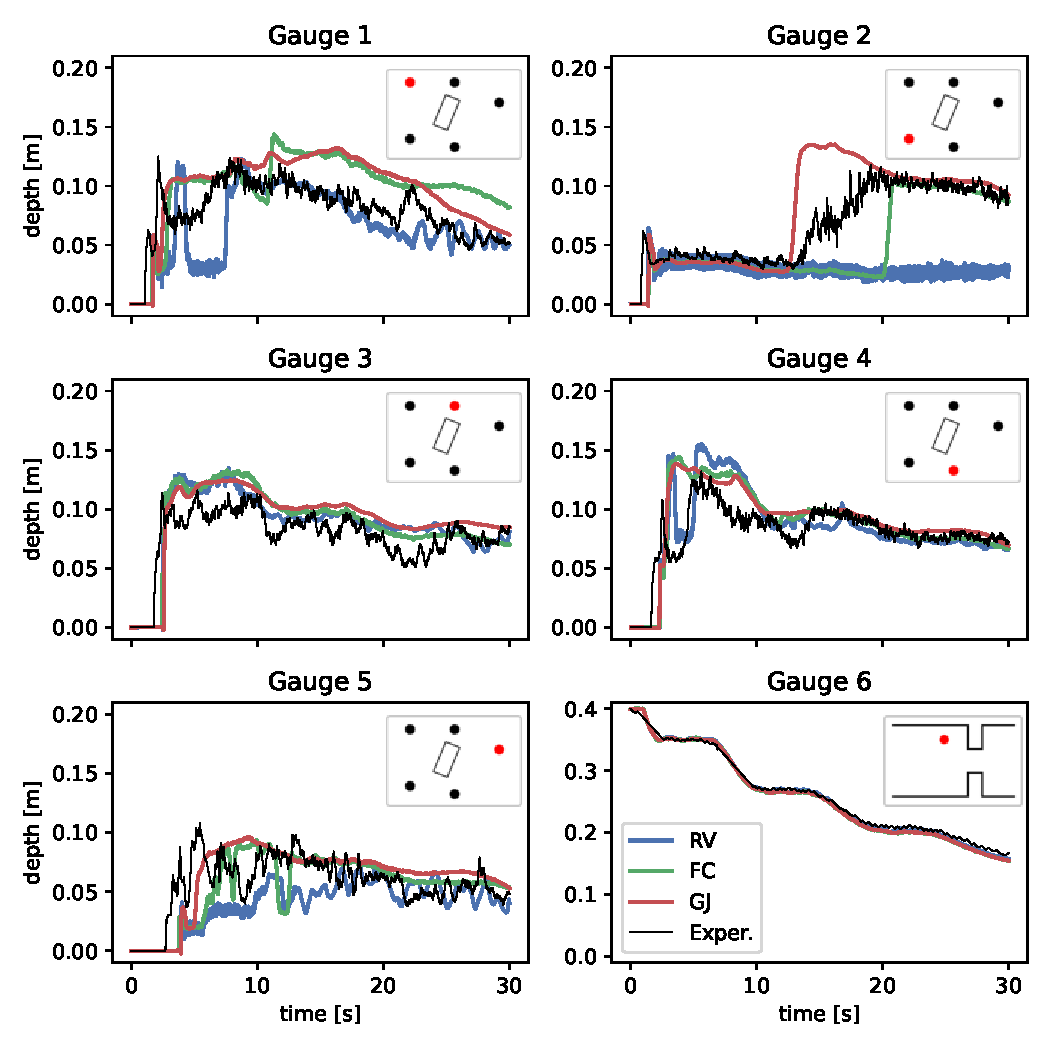
\includegraphics[width=\textwidth]{img/eulerian/exp/gauges.pdf}
\caption{Experimental dam break flow. Comparison between the obtained water depth with the reference data.}
\label{experiment_gauges}
\end{figure}

Gauge 3 is located at the left hand side of the building, where multiple waves are reflected and practically always it is in subcritical regime. There is a good correlation between numerical and experimental results. Gauge 4 is at the opposite side of the building but the superposition of the reflected waves is more clearly identified. The main discrepancies in the results are concentrated in the first seconds, where the flow is more dynamic.

Gauge 6 is located at the reservoir and registers the superposition of smooth waves during the emptying of the tank.

As stated in \cite{soares2007} there are some difficulties in the recording of the velocity and its validity is discussed. Here we compare only the most representative gauges. Gauge 2 is not fully submerged and the validity of the measurements is good after $t=14.5s$. It illustrates the change from supercritical flow to subcritical (Figure \ref{experiment_gauge2_vel}). The considerations are similar to the water depth study.


\begin{figure}
\centering
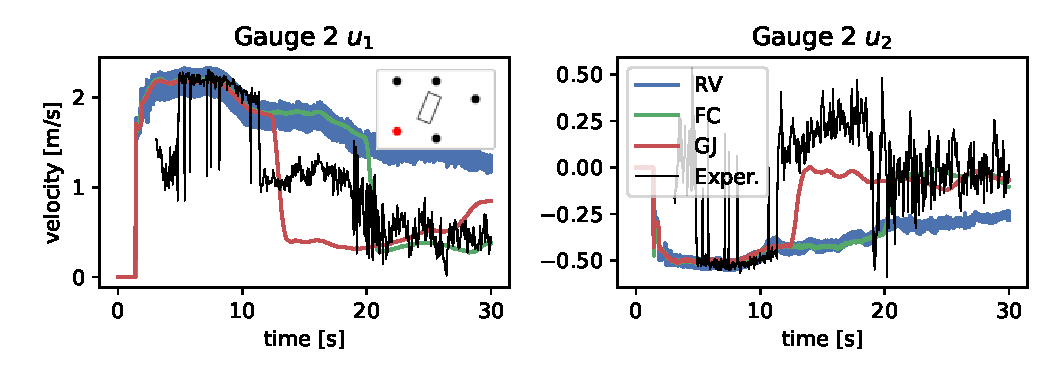
\includegraphics[width=\textwidth]{img/eulerian/exp/gauge2_vel.pdf}
\caption{Experimental dam break flow. Comparison of velocity at gauge 2.}
\label{experiment_gauge2_vel}
\end{figure}

The experimental measurements in gauge 4 (Figure \ref{experiment_gauge4_vel}) show a change in the velocity direction around $t=15s$ due to the rise of water level. The numerical results do not capture this change but the mean and the stationary values are correctly simulated.

\begin{figure}
\centering
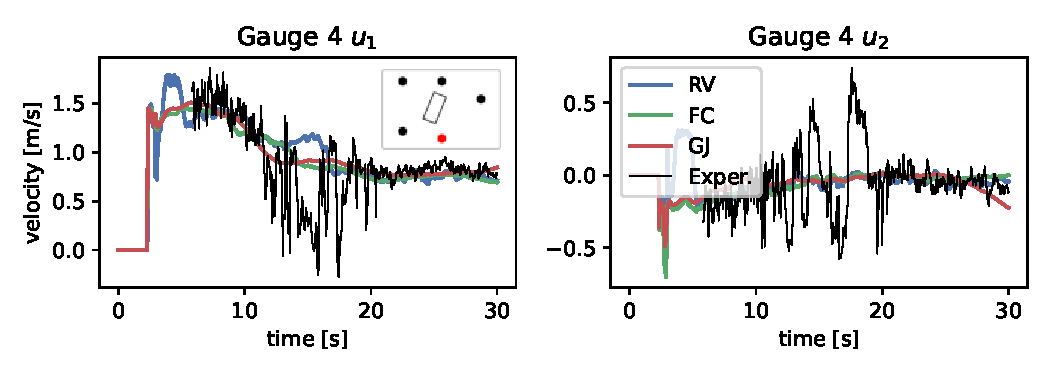
\includegraphics[width=\textwidth]{img/eulerian/exp/gauge4_vel.pdf}
\caption{Experimental dam break flow. Comparison of velocity at gauge 4.}
\label{experiment_gauge4_vel}
\end{figure}

In gauge 5 the formation of eddies behind the building can be appreciated from $t=20$ (Figure \ref{experiment_gauge5_vel}). In that case, the experimental results have difficulties to capture the eddies. Results will probably improve by extending the refined region of the mesh. The authors have observed the formation of eddies, but they are not fully developed and its area of influence is not enough to arrive to gauge 5.


\begin{figure}
\centering
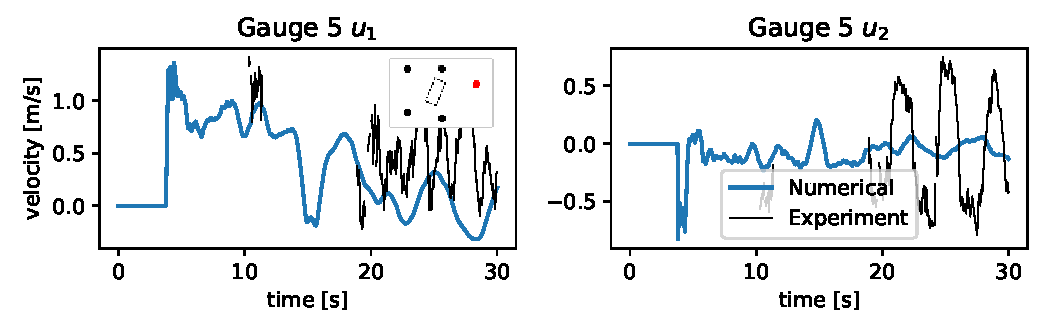
\includegraphics[width=\textwidth]{img/eulerian/exp/gauge5_vel.pdf}
\caption{Experimental dam break flow. Comparison of velocity at gauge 5.}
\label{experiment_gauge5_vel}
\end{figure}


In fluid-structure interaction studies, pressure is needed to compute to forces over the structure. The shallow water assumptions drop the dynamic pressures retaining only the hydrostatic ones. In the present case, the pressures are recovered by integrating the hydrostatic pressures given the water depth around the building. However, there is no experimental data about the forces applied to the building and thus, the importance of the dynamic pressures can not be evaluated.


Regarding the performance of the FIC-FEM formulation, it captures the main aspects of the flow, but not the details, since there are some regions on that experiment which violate the shallow water approximations.










\section{The flux corrected transport for the shallow water equations}
\label{sec:fc}



As seen before, the numerical approximation of hyperbolic systems -convection dominant- exhibits instabilities. Those instabilities are inherent to schemes of order greater than 1 (Godunov barrier theorem \cite{godunov1959}). With the aim of suppressing the spurious oscillations and to extend to stable schemes to higher orders, the flux corrected algorithms were proposed.
This new family of methods seeks for non oscillatory solutions and also for monotonicity of the numerical solution. At first, the flux corrected algorithms were proposed for structured meshes and explicit time integration schemes \cite{boris1973, book1975}. Generally, they were based for FD algorithms, but rapidly were extended also to Galerkin discretizations and implicit schemes \cite{kuzmin2001, lohner2008ch9}. Even though, the flux corrected transport has not been extended to many applications in the FEM community.


In this section the concept of flux correction is extended to the SW equations. The linearized equations presented in Chapter \ref{equations} can be understood as a generalization of the scalar transport equations, where the convection operator is extended with a matrix and the scalar unknown is replaced by a vector. This extension is proposed as an alternative to Lagrangian methods (Chapter \ref{lagrangian_sw}), where the shoreline discontinuity is naturally captured. At the same time, looks for a better accuracy than the stabilized Eulerian methods (Section \ref{sec:fic_fem_stabilization}):
the introduction of the \emph{shock capturing} leads to a lower convergence order, making them first order. The main purpose to explore the flux corrected algorithm is to make the numerical solution inherit the monotonicity of the physical solution. The water column is a positive property, whereas null water depth means the dry sub-domain.
Tracking the zero isoline properly is of crucial importance to accurately model the wetting and drying processes -floods-. Unfortunately, the zero isoline presents a discontinuity in the unknowns and the hyperbolic property is lost, leading to numerical oscillations and consequently, losing the monotonic property.


The flux corrected algorithm is based on the modification of the resulting matrices from the discrete weak variational. The formulation presented in Section \ref{sec:fic_fem} will be modified in order to enforce it to verify monotonic properties at the discrete level. The subjacent correction acts such way that all the modifications are conservatives, namely, there is not gain or loss of fluid mass. The original scheme is recovered where the solution is smooth and does no require modifications.


In order to achieve that properties, the low order scheme is constructed through a lumping procedure of the mass matrix and the addition of enough diffusion in order to eliminate the negative entries of the off-diagonal terms. In that way, the construction of the low and high order schemes is performed elementally. On the other hand, the computation of the fluxes and its limiters is computed nodally. Finally, the global assembly is element-wise, as far as the nodes belong to the elements. The fact of recovering the high order scheme ith consistent mass matrix is specially interesting to accurately simulate transient problems.




\subsection{Equivalence with pure convection problems}

In a first instance, the flux corrected algorithms where developed for the transport equations as a two stage predictor-corrector algorithm. The correction of the fluxes had a direct relation with the physical fluxes and were evaluated at the edges of the mesh, acting directly to the entries of the global matrix.

Since the pure convection problem is a particular hyperbolic system of conservation law, this algorithm was extended to more complex systems, like the Euler equations. Here we will show the equivalence of the inviscid SW equations with pure convection problems.
The starting point are the linearized SW equations in conservative form (\ref{general_sw_lin}), which are analogue to the hyperbolic euler equations:

\begin{equation}
\pder{\bm\phi}{t} + \bm A_i \pder{\bm\phi}{x_i} = 0
\end{equation}

The matrix $\bm A_i$ is diagonalizable and can be decomposed as $\bm A_i = \bm T_i \bm\Lambda_i \bm T_i^{-1}$. Kuzmin \cite{kuzmin2005b} proposes a transformation for the one dimensional case. In high order dimensions, we can define a vector of transformed unknowns $\bm\Phi_i = \bm T_i^{-1}\bm\phi$ which yields


\begin{equation}
\pder{\bm\Phi_j}{t} + \bm\Lambda_i \pder{\bm\Phi_j}{x_i} = 0
\end{equation}
Since $\bm\Lambda$ is a diagonal matrix, the above expression consists on a set of decoupled convection equations.

\begin{equation}
\pder{\Phi_{jk}}{t} + \Lambda_{ikk} \pder{\Phi_{jk}}{x_i} = 0 , \quad
k = 1,\text{dim}+1 , \quad
i,j = 1,\text{dim}
\end{equation}

In practice, instead of applying the flux correction concept to the diagonal system, the algorithm will be extended to the original system os equations. The main difficulty which appears when the system is decomposed is that there isn't a unique direction of propagation for each uncoupled unknowns. This is known as the dispersive behavior of the shallow water equations.



\subsection{FCT algorithm}

The FCT algorithm inherits the concept of limiting introduced by Boris and Book \cite{boris1973} and was developed by Löhner \cite{lohner2008ch9} and Kuzmin \cite{kuzmin2001}. They also extended the concept of flux correction for transport schemes to the euler equations \cite{lohner2008ch9, kuzmin2005b}. In more recent developments, the flux correction techniques are applied to the shallow water equations, see Ortiz \cite{ortiz2012}. However, Ortiz presents an algorithm with fully decoupled high and low order solutions. In this section, the flux corrected scheme is applied to the shallow water equations preserving the same discretization for both high and low order solutions. 



\subsubsection{High and low order schemes}

The high order solution uses the spatial discretization presented in [FIC-based shallow water eq.] and the backward differentiation formula for the time integration.

\begin{equation} \label{ho}
\mathbf{M}_C\dot{\phi}^{n+1} + \mathbf{K}\phi^{n+1} = \mathbf{q}
\end{equation}
\begin{equation} \label{bdf}
\dot{\phi}^{n+1} = \beta_1\phi^{n+1} + \beta_2\phi^{n} + \beta_3\phi^{n-1}\dots
\end{equation}

where $\phi$ is the vector of the nodal unknowns and $\dot{(\ )}$ denotes the time derivative, $\mathbf{M}_C$ is the consistent mass matrix, $\mathbf{K}$ is the system matrix and $\mathbf{q}$ is the source term. This scheme will be taken as reference for the high order scheme but, as any stabilized and not monotonicity preserving formulation, is not oscillation-free, specially near the wet-dry interface.
%In \cite{ortiz2012} the high order solution is obtained with the CBS algorithm, which was initially proposed by Zienkiewicz and Taylor \cite{zien3}.

The low order solution is obtained from the high order scheme with a mass lumping procedure and adding scalar diffusion to the high order scheme:

\begin{equation} \label{lo}
\mathbf{M}_L\dot{\phi}^{n+1} + \left(\mathbf{K+D}\right)\phi^{n+1} = \mathbf{q}
\end{equation}
\begin{equation} \label{scalar_diffusion}
\mathbf{D} = c_\tau\left(\mathbf{M}_L - \mathbf{M}_C\right)
\end{equation}

The difference between the two systems of equations is the amount of artificial diffusion which ensures monotonicity and can be formally written as

\begin{equation}
\mathbf{P}(\phi^{n+1}, \phi^n) = (\mathbf{M}_L - \mathbf{M}_C)\dot{\phi}^{n+1} - \mathbf{D} \phi^{n+1}
\end{equation}

Following Kuzmin \cite{kuzmin2005a}, one can observe that the anti-diffusion $\mathbf{P}$ can be decomposed into a sum of internodal fluxes $f_{ij}$ where the contribution to node $i$ from the node $j$ is the opposite from $i$ to $j$, that is $f_{ij}=-f_{ji}$. This edge-based approach shows that the quantity added to a node, is subtracted from another node, and the anti-diffusion is conservative. For convenience we will keep the finite element structure. The high order scheme is recovered if the unlimited correction $\mathbf{P}$ is added to the low order scheme.



\subsubsection{Flux correction}

The essentials of the flux corrected method is to switch between the low and high order solutions in an adaptive fashion to satisfy the positivity constraint. The Zalesak's limiter is employed to define the amount of anti-diffusion added to the low order solution which at the same time guarantee the positivity constraint for a given variable.

The antidiffusive fluxes are decomposed in those that increase the value and those that decrease it, the increment $\mathbf{P}_i$ is decomposed in a sum of positive and negative contributions

\begin{equation}
P_i = P_i^+ + P_i^- \ , \qquad
P_i^{\pm} = \sum_{j\neq i} \,
_{\min}^{\max} \{0, j_{ij}\}
\end{equation}

While the maximum/minimum admissible increments depends on the solution values at the neighboring nodes that share an element with node $i$

\begin{equation} \label{admissible_increment}
Q_i^\pm =\, _{\min}^{\max}\Delta \phi_{ij}^\pm \ , \qquad
\text{where} \quad \Delta \phi_{ij}^\pm =\, _{\min}^{\max}
\{0, \tilde{\phi}_j - \tilde{\phi}_i\}
\end{equation}

where the $\tilde{(\ )}$ symbol denotes a predictor for the solution at time $t^{n+1}$. In order to prevent the formation of spurious oscillations, the positive/negative anti-diffusive flux should be limited by the following ratio

\begin{equation}
R_i^\pm = \begin{cases}
    \min\{1, Q_i^\pm / P_i^\pm\} & \text{if} P_i^\pm \neq 0 \\
    1 & \text{if} P_i^\pm = 0
\end{cases}
\end{equation}

Note that in order to preserve mass conservation property the same limiter should be applied to all the element contributions, the most restrictive ratio is chosen:

\begin{equation}
c_e = \min\{R_i^\pm\}\ , \quad \forall \text{node}_i \in \text{element}_e
\end{equation}

% \begin{equation}
% c_e = \begin{cases}
%     \min\{R_i^+\} & \quad \text{if} \quad \sum_i f_i>0 \\
%     \min\{R_i^-\} & \quad \text{if} \quad \sum_i f_i<0
% \end{cases}
% \end{equation}



\subsubsection{Iterative solution}

Since the linearization matrix $A$ depends on the solution at time $t^{n+1}$, the system matrix $K$ needs to be updated at the end of each iteration and the low order algebraic system of equations (\ref{lo}) is rewritten in residual based form

\begin{equation} \label{residual_based}
\left(\beta_0 \mathbf{M}_L + \mathbf{K}^{(m)} + c_\tau\mathbf{D}\right) \Delta\phi^{(m+1)} =
\mathbf{q} - \left(\mathbf{K}^{(m)} + c_\tau\mathbf{D}\right)\phi^{(m)}
-\mathbf{M}_L\dot{\phi}^{(m)}
\end{equation}

where $\phi^{(0)} = \phi^n$. After adding the limited flux correction and substitutions, the system (\ref{residual_based}) yields

\begin{multline}
\left(\beta_0 (c\mathbf{M}_c + (1-c)\mathbf{M}_L)
    + \mathbf{K}^{(m)} + c_\tau(1-c)\mathbf{D}\right) \Delta\phi^{(m+1)} = \\
\mathbf{q} -\left( \mathbf{K}^{(m)} + c_\tau(1-c)\mathbf{D} \right) \phi^{(m)}
    - \left(c\mathbf{M}_c + (1-c)\mathbf{M}_L \right) \dot{\phi}^{(m)}
\end{multline}




NOTE: the displacement or residual criteria does not converge if the $c_i$ limiter vary along the iterations $(m)$. There are some alternatives to overcome this issue:
\begin{itemize}
    \item to use a constant $c_i$, obtained from the first iteration. This solution may not be optimal and possibly does not preserve monotonicity;
    \item to use a semi-implicit time integration scheme which defines the predictor $\tilde{\phi}$ see equation (\ref{admissible_increment});
    \item to define an incremental limiting, this seems to be the most accurate scheme, even though it is more diffusive than the presented one.
\end{itemize}



\subsubsection{Limiting a set of equations and variable transformation}

The presented limiting is based on the monotonicity requirements for scalar convection, however, the coupling of the shallow water equations require a synchronized limiting for the correction factors. It is commonly accepted that for coupled systems of equations the flux limiter taken the most restrictive among the set of variables $c_i^+ = \min\{c_{ik}^+\}$ and $c_i^- = \min\{c_{ik}^-\}$. There are the following strategies to compute the set of limiters $c_{ik}^\pm$:

\begin{itemize}
    \item flux limiting in terms of the independent variables $h, \mathbf{q}$;
    \item flux limiting based on several indicators as the total energy, water pressure or maximum eigenvalue;
    \item transformation of the variables into characteristic variables in order to obtain a set of decoupled system of equations where the principles of the flux correction for pure convection can be applied.
\end{itemize}

In omission of source terms, equation (\textcolor{red}{EQ RESIDUAL}) can be multiplied by the $\mathbf{T}_i$ base of eigenvectors and transformed into a set of decoupled pure convection problems

\begin{equation}
\pder{\Phi_{jk}}{t} + \Lambda_{ikk} \pder{\Phi_{jk}}{x_i} = 0 , \quad
k = 1:\text{dim}+1 , \quad
i,j = 1:\text{dim}
\end{equation}

This transformation can be computed locally at each node and depends on the current solution at time $t^{n+1}$. However, for the two dimensional case, the set of variables $\phi$ is transformed in a two dimensional vector of variables $\Phi_i$, hence the scalar transport correction techniques should be extended to vectorial transport.



NOTE: This transformation requires more study, specially for the convection of vectors and the corresponding flux correction technique.


\subsection{Examples}

Incorporar los resultados...


\subsection{Concluding remarks}

Importancia de que la solución de bajo orden esté estabilizada. En caso contrario, aparecen fenómenos de "terraza" o un exceso de difución y dependencia de la malla.

Dificultad de definir el criterio de convergencia. Incluso cuando se comparan los incrementos diferenciales (desplazamientos) de la solución, no se alcanza una convergencia razonable. Probablemente, este estancamiento de la solución se debe a una oscilación en las correcciones añadidas.

Coste computacional. Aunque el algoritmo tiene que resolver un sistema con el mismo número de grados de libertad que un esquma con estabilización lineal (\ref{sec:fic_fem_stabilization}), la introducción de las correcciones es no lineal. Esta no linealidad supone un coste copmutacional adicional, ya que requiere un número muy superior de iteraciones. Una posibilidad sería limitar el número de iteraciones a un número fijo, por ejemplo, 4. Sin embargo, no se tendría un control de la precisión obtenida ante problemas transitorios, donde la presencia de obstáculos en el fluido y fenómenos altamente dinámicos, pueden requerir de más iteraciones para obtener un resultado satisfactorio.

Buenos resultados observando la solución, sin embargo, el orden de convergencia no es el deseado.



\section{Quasi monotonicity preserving formulations}



\section{Stabilized formulation for the Boussinesq modified equations}




\subsection{Absorbing boundary conditions}

Es frecuente que que sea necesario acotar el dominio de estudio, imponiendo condiciones abiertas. Estas condiciones de contorno abiertas o radiantes han de permitir la salida de ondas, al mismo tiempo que garantizan la consistencia matemática del sistema de ecuaciones. Al mismo tiempo que la expresión matemática ha de garantizar la existencia de la solución, tambień ha de ser compatible con la disretización numérica empleada para el interior del dominio. Generalmente, se denomina condiciones de contorno radiantes a la formulación analítica y condiciones de contorno absorbentes al método numerico \cite{navon2004}.
Se busca un equilibrio entre la precisión con la que se aproxima la condición de radiación (reducción de reflexión) y el coste computacional.

En este sentido, es de gran importancia que el método numérico junto con las condiciones escogidas, resulten en un esquema estable, al mismo tiempo que las oscilaciones espúreas generadas por la reflexión sean pequeñas.
Por otro lado, hay que asegurar que el cálculo de las condiciones de contorno no concluyan en un coste computacional excesivo comparado con el del dominio interior.

La primera consideración es que, tomando $\eta$ como la superficie libre y en un caso unidireccional, una función de onda presentará una condición radiante donde verifique que
\begin{equation} \label{radiation_condition}
    \pder{\eta}{t} + c \cos(\theta)\pder{\eta}{x} = 0
\end{equation}
donde $\eta$ es la variación de la superficie libre, expresada en términos del calado $h$ y la topografía $z_b$, $c$ es la velocidad de propagación de las ondas y $\theta$ es el ángulo con la frontera.

Algunos autores como Engquist propusieron aproximaciones locales altamente disipativas \cite{engquist1977}, más adelante Bayliss \cite{bayliss1982} exploró las condiciones radiantes para las ecuaciones de Helmholtz. De modo similar, Collino \cite{collino1993} extendió la formulación empleando derivadas de mayor orden. Sin embargo, la generalización para las ecuaciones de Euler o, análogamente, a las ecuaciones de aguas poco profundas en 2D no es trivial. Por un lado, el ángulo de incidencia $\theta$ no es conocido \emph{a priori}, dando lugar a la reflexión de la componente no alineada. Por otro lado, las ecuaciones de aguas poco profundas son disperivas y no hay una sola celeridad que caracterice el sistema \cite{wei1995}. Es decir, hay tres ondas superpuestas que se propagan con velocidades diferentes. Por ejemplo, se pueden reescribir las ecuaciones \ref{general_sw} en variables características, mediante la diagonalización de la matrices tangentes $\mathbf{A}_i$ de la forma
\begin{equation}
    \pder{\bm\Phi_j}{t} + \bm\Lambda_i \pder{\bm\Phi_j}{x_i} = 0
\end{equation}
donde $\bm\Lambda$ es una matriz diagonal tal que $\bm A_i = \bm T_i \bm\Lambda_i \bm T_i^{-1}$. El problema resultante es la conveción de tres ondas, cada una asociada a las velocidades $\lambda_i$, que corresponden a $u-c$, $u$ y $u+c$. Los distintos valores de $\lambda_i$ determinan si cada condición de contorno se trata de una entrada o salida, y si es sub-crítica o super-crítica.

A parte de tener que imponer la condición radiante para las tres ondas, la validez de este método es limitada, ya que en más de 1D no existe una formulación genuina basada en caracterísitcas. Puede encontrarse un desarrollo completo en \cite{lie2001}.

Muchas de las aproximaciones propuestas \cite{israeli1981,navon2004,carmigniani2018} consisten en relajar la condición (\ref{radiation_condition}) añadiendo un término disipador $K$
\begin{equation} \label{radiation_absorbing_condition}
    \pder{\eta}{t} + c \cos(\theta)\pder{\eta}{x} = -K\eta
\end{equation}
y extendiendo el dominio en una distancia $d$. Esta aproximación se suele emplear en combinación con condiciones absorbentes locales \cite{wei1995}.

Otra de las vías exploradas es la Perfectly Matched Layer (PML) \cite{berenger1994}, que ha sido ampliamente utilizada en la literatura. Presenta el inconveniente de tener que imponer tratamietos especiales en las esquinas.

Posteriormente, esta metodología fue empleada en combinación con las fronteras absorbentes de alto orden, dando lugar a la Double Absorbing Boundary (DAB), propuestas por Hagstrom y Rabinovich \cite{hagstrom2014,rabinovich2015}. Esta úlima metodología ubica dos fronteras paralelas, separadas por una pequeña distancia. Presenta la ventaja de no tener que incorporar derivadas en la dirección normal ni tener que aplicar tratamientos especiales a las esquinas.

Dada la simplicidad de la formulación, se ha optado por introducir solamente una capa de esponja, sigiendo las formulaciones de \cite{israeli1981} y \cite{carmigniani2018}. Se ha introducido un factor disipador Newtoniano de la siguiente forma análogo a la fricción de fondo $S_f$ de la siguiente forma:
\begin{equation}
    S_a = -\gamma(\mathbf{x}) \mathbf{u}
\end{equation}


El término disipador $\mathbf{\gamma}$ varía desde cero hasta al valor máximo $\gamma_{\max}$ junto a la frontera. Sigue un ley exponencial \cite{peric2018} que depende del exponente $n$. Los parámetros del grosor de la esponja $d_0$ y valor máximo deben determinarse para casa caso, según la longitud de onda de las olas.

\begin{equation} \label{exponential_sponge_layer}
    \gamma(\mathbf{x}) = \gamma_{\max} \mathcal{H}(d_0 - d(\mathbf{x})) \frac{e^{\left(\frac{d_0 - d(\mathbf{x})}{d_0}\right)^n} - 1}{e - 1}
\end{equation}
where $\mathcal{H}$ is the Heaviside function, $d$ is the distance from a point to the computational boundary.

En la figura \ref{absorbing_boundary} se muestra la propagación de un tren de olas mono-cromáticas. En un extremo del dominio se generan las olas, en el extremo opuesto hay una frontera absorbente. Estudios como el realizado por \cite{carmigniani2018} muestran que diversos valores de absorción, grosor de la esponja, o de la función exponencial (\ref{exponential_sponge_layer}) pueden provocar reflexiones no deseadas. Por ejemplo, una excesiva absorción provocaría una reflexión al inicio de la capa de esponja.

Se ha elegido $n=3$ para la expresión (\ref{exponential_sponge_layer}), por ser un valor que minimiza considerablemente la reflexión (ver \cite{carmigniani2018}). Queda hacer un análisis de sensibilidad de los parámetros $d_0$ y $\gamma_{\max}$.

Resulta práctico expresarlos en términos relativos a la longitud de onda $\lambda$ y a la frecuencia $\omega$. En la práctica, el grosor de la capa esponja suele ser $d_0 \approx 2\lambda$ y el coefficiente de absorción $\gamma \approx 0.5\omega$. Mientras que el coeficiente de reflexión es monótono decreciente con grosor de la capa, presenta un mínimo local respecto a la frecuencia. Esto hace que para un tren de olas sea recomendable ajustar los parámetros de acuerdo con la máxima longitud de onda.


\begin{figure}
    \centering
    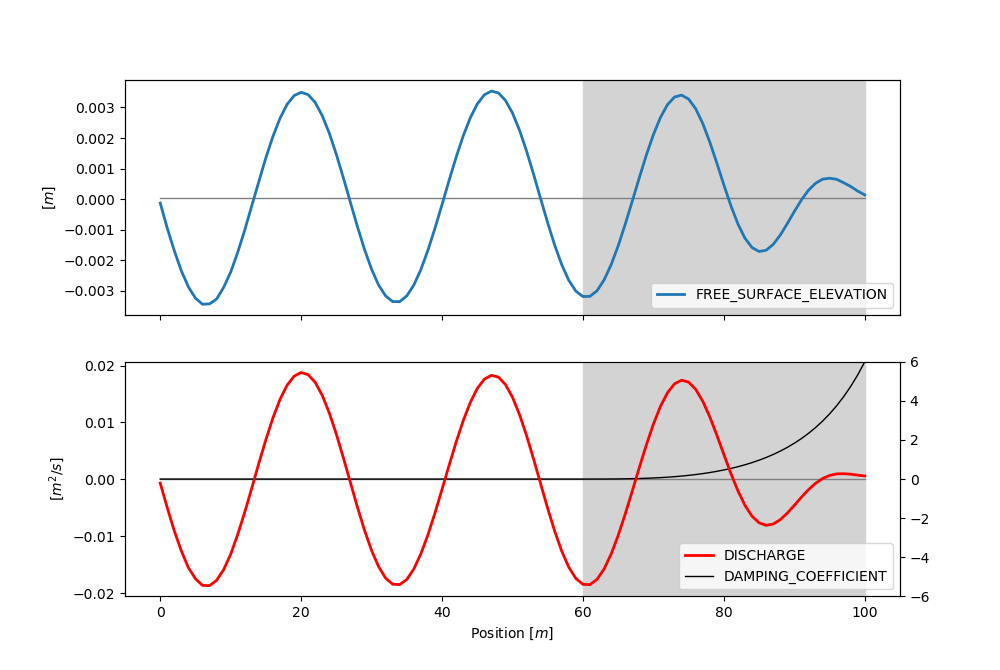
\includegraphics[width=.8\textwidth]{img/absorbing_boundary.png}
    \caption{Propagación y absorción de un tren de olas. La región sombreada de gris muestra el grosor de la capa esponja.}
    \label{absorbing_boundary}
\end{figure}


\subsection{Examples}



\section{Concluding remarks}


